\documentclass{dreamlab-business}

\usepackage{booktabs}
\usepackage{graphicx}
\usepackage{tikz}
\usepackage{pgfplots}
\pgfplotsset{compat=1.17}
\usepackage{hyperref}
\usepackage{enumitem}
\usepackage{amsmath}
\usepackage{eurosym}

% Document metadata
\title{DreamLab AI Consulting}
\subtitle{Comprehensive Business Plan \& Property Development Strategy}
\author{Executive Team}
\date{July 2025}

\makeindex

\begin{document}

\maketitle
\tableofcontents

% --- Automatically include all section .tex files for a comprehensive report ---
\begin{executivesummary}
DreamLab AI Ltd represents a pioneering convergence of creative technology, agentic engineering, and advanced simulation in a residential training environment. Located on a 1.5 acre plot in Eskdale Green, Cumbria, 10 minutes drive from Sellafield Nuclear Storage and Processing, our facility bridges the gap between artistic vision, autonomous systems, and technical precision through immersive, hands-on learning experiences. Our unique business model combines:

\begin{itemize}
    \item \textbf{Creative Technology Hub}: State-of-the-art virtual production facility with a media and AI lab.
    \item \textbf{Target Audience}: Decision makers in diverse industries, with small cohort sizes of 3-6.
    \item \textbf{Accommodation}: 3 bedrooms, a kitchen, a gym, and a sauna, available for corporate training or rental to the mobile engineering community and families.
\end{itemize}

\subsection*{Key Investment Highlights}

% [Moved KPI graphics after summary]

\subsection*{Strategic Advantages}

\begin{enumerate}
    \item \textbf{Market Innovation}: First UK facility combining virtual production, agentic engineering, and simulation
    \item \textbf{Technology Leadership}: Cutting-edge equipment including 6m LED volume, agent development cluster, and gaussian splatting rigs
    \item \textbf{Industry Expertise}: Leadership team from Oscar-winning studios, AI pioneers, and Fortune 500 tech companies
    \item \textbf{Geographic Advantage}: Wales location offers 40\% cost savings vs London with government innovation support
    \item \textbf{Future-Proof Focus}: Agentic systems represent the next wave of AI adoption across all industries
\end{enumerate}

\subsection*{Market Opportunity}

% [Moved market table after summary]

\subsection*{Revenue Model Evolution}

% [Moved revenue pie chart after summary]

\subsection*{Financial Summary}

% [Moved financial summary table after summary]

\subsection*{Investment Requirements}

Total capital requirement: \pounds{950,000}
\begin{itemize}
    \item Phase 1 (Virtual Production Setup): \pounds{350,000}
    \item Phase 2 (Agentic Engineering Lab): \pounds{200,000}
    \item Phase 3 (Simulation \& Compute): \pounds{200,000}
    \item Phase 4 (Accommodation \& Sustainability): \pounds{150,000}
    \item Phase 5 (Working Capital): \pounds{50,000}
\end{itemize}

\subsection*{Use of Funds}

\begin{center}
\begin{tikzpicture}[scale=0.8]
    \pie[color={dreamlab-purple, dreamlab-blue, dreamlab-green, dreamlab-orange, dreamlab-grey}]{
        37/Creative Tech Infrastructure,
        21/Agentic Engineering Lab,
        21/Computing \& Simulation,
        16/Facility Development,
        5/Working Capital
    }
\end{tikzpicture}
\end{center}

\subsection*{Unique Value Propositions}

\begin{enumerate}
    \item \textbf{Agentic Engineering Leadership}: First dedicated facility for hands-on agent development training
    \item \textbf{Creative-Technical Convergence}: Where Hollywood meets engineering simulation
    \item \textbf{Residential Immersion}: Deep learning away from daily distractions
    \item \textbf{Equipment Access}: \pounds{2.5M} of specialized hardware available to students
    \item \textbf{Industry Connections}: Direct pathways to employment and partnerships
\end{enumerate}


\end{executivesummary}
\section{Company Overview}

\subsection{Vision and Mission}

\begin{keypoint}
\textbf{Vision}: To become the UK's premier destination for immersive AI learning experiences, where cutting-edge technology meets sustainable living.

\textbf{Mission}: Empowering professionals and organisations with practical AI skills through hands-on training in an inspiring, eco-conscious environment that demonstrates the harmony between technological advancement and environmental stewardship.
\end{keypoint}

\subsection{Company Structure}

DreamLab AI Ltd is a private limited company registered in England (Wilmslow, Manchester), focusing on technology and training services. A separate sole trader entity, registered in Cumbria, will manage the eco-luxury accommodation and related services.

The business specialises in:
\begin{itemize}
    \item Advanced AI/ML training and consultancy services
    \item Sustainable technology demonstrations
    \item Eco-luxury holiday accommodation and corporate retreats
\end{itemize}

\subsection{Founding Team}

The company is led by a single founder, with a flexible model of bringing in specialist contractors and partners on a per-project basis to meet specific client needs.

\subsection{Legal Structure and Governance}

\begin{itemize}
    \item \textbf{Company Type}: Private Limited Company (Ltd)
    \item \textbf{Registration}: Companies House England
    \item \textbf{VAT Status}: Registered for both training services and accommodation
    \item \textbf{Insurance}: Professional indemnity, Public liability, Property insurance
    \item \textbf{Certifications}: ISO 27001 (planned), Cyber Essentials Plus
\end{itemize}

\subsection{Strategic Partnerships}

DreamLab will collaborate with a network of partners to deliver its vision:
\begin{itemize}
    \item \textbf{Technology Providers}: Partnerships with leading hardware and software companies like NVIDIA, Microsoft Azure, and OpenAI to ensure access to cutting-edge tools.
    \item \textbf{Simulation and Virtual Production}: Collaborations with virtual production studios and simulation technology providers across the UK.
    \item \textbf{Academic Institutions}: Engaging with universities for research collaboration and talent development.
    \item \textbf{DreamLab Collective}: Leveraging the expertise of the wider DreamLab network of specialists and consultants.
    \item \textbf{Industry Bodies}: Working with organisations like the UK AI Council to align with national standards and policy.
\end{itemize}

\subsection{Competitive Advantages}

\begin{center}
\begin{tikzpicture}[node distance=2cm]
    % Central node
    \node[circle, draw=dreamlab-purple, fill=dreamlab-lightgrey, minimum size=3cm, align=center] (center) {\textbf{DreamLab}\\\textbf{Advantages}};

    % Surrounding advantages
    \node[rectangle, draw=dreamlab-blue, fill=dreamlab-lightblue!20, align=center, above=of center] (adv1) {Unique Dual\\Revenue Model};
    \node[rectangle, draw=dreamlab-green, fill=dreamlab-green!20, align=center, right=of center] (adv2) {Hands-on\\Lab Equipment};
    \node[rectangle, draw=dreamlab-orange, fill=dreamlab-orange!20, align=center, below=of center] (adv3) {Sustainable\\Operations};
    \node[rectangle, draw=dreamlab-grey, fill=dreamlab-grey!20, align=center, left=of center] (adv4) {Rural Location\\Benefits};

    % Connect nodes
    \draw[->] (center) -- (adv1);
    \draw[->] (center) -- (adv2);
    \draw[->] (center) -- (adv3);
    \draw[->] (center) -- (adv4);
\end{tikzpicture}
\end{center}

\subsection{Core Values}

\begin{enumerate}
    \item \textbf{Innovation}: Pioneering new approaches to AI education
    \item \textbf{Sustainability}: Demonstrating environmental responsibility
    \item \textbf{Accessibility}: Making AI training available to diverse audiences
    \item \textbf{Excellence}: Delivering exceptional learning experiences
    \item \textbf{Community}: Building lasting relationships with learners and partners
\end{enumerate}
\section{Market Opportunity}

\subsection{AI Training Market Analysis}

The global AI training market is experiencing unprecedented growth, driven by digital transformation across all sectors:

\begin{table}[H]
\centering
\begin{tabular}{lrr}
\toprule
\textbf{Market Segment} & \textbf{2024 Value} & \textbf{2028 Projection} \\
\midrule
Global AI Training Market & \$4.2 billion & \$12.8 billion \\
UK AI Training Market & \pounds{320} million & \pounds{980} million \\
North West Tech Training & \pounds{50} million & \pounds{150} million \\
Corporate AI Education & \$2.1 billion & \$7.5 billion \\
\bottomrule
\end{tabular}
\caption{AI Training Market Projections (Source: Gartner, IDC)}
\end{table}

\subsection{Target Market Segments}

\subsubsection{Primary Markets}

\begin{enumerate}
    \item \textbf{Corporate Training} (60\% of revenue)
    \begin{itemize}
        \item Large enterprises seeking AI upskilling
        \item SMEs requiring AI integration support
        \item Government departments and public sector
        \item Financial services and insurance companies
    \end{itemize}

    \item \textbf{Individual Professionals} (25\% of revenue)
    \begin{itemize}
        \item Software developers transitioning to AI
        \item Data scientists seeking practical experience
        \item Business analysts learning AI applications
        \item Consultants expanding service offerings
    \end{itemize}

    \item \textbf{Holiday Lettings} (15\% of revenue)
    \begin{itemize}
        \item Tech professionals seeking working holidays
        \item Eco-conscious travellers
        \item Digital nomads requiring high-speed connectivity
        \item Weekend retreat guests
    \end{itemize}
\end{enumerate}

\subsection{Market Trends and Drivers}

\begin{center}
\begin{tikzpicture}
    \begin{axis}[
        title={UK AI Skills Demand Growth},
        xlabel={Year},
        ylabel={Job Postings Requiring AI Skills (thousands)},
        xmin=2020, xmax=2028,
        ymin=0, ymax=300,
        xtick={2020,2022,2024,2026,2028},
        ytick={0,50,100,150,200,250,300},
        legend pos=north west,
        ymajorgrids=true,
        grid style=dashed,
    ]

    \addplot[
        color=dreamlab-purple,
        mark=square,
        line width=2pt
    ]
    coordinates {
        (2020,45)(2021,68)(2022,95)(2023,125)(2024,165)(2025,195)(2026,235)(2027,265)(2028,290)
    };
    \addlegendentry{AI Skills Demand}

    \addplot[
        color=dreamlab-blue,
        mark=o,
        line width=2pt
    ]
    coordinates {
        (2020,30)(2021,38)(2022,45)(2023,55)(2024,68)(2025,82)(2026,98)(2027,115)(2028,135)
    };
    \addlegendentry{Available AI Professionals}

    \end{axis}
\end{tikzpicture}
\end{center}

\subsection{Competitive Landscape}

\begin{table}[H]
\centering
\begin{tabularx}{\textwidth}{lXcc}
\toprule
\textbf{Competitor} & \textbf{Strengths} & \textbf{Lab Facilities} & \textbf{Accommodation} \\
\midrule
Online Platforms & Wide reach, Low cost & No & No \\
University Courses & Academic credibility & Limited & No \\
Tech Bootcamps & Intensive learning & Sometimes & No \\
Corporate Training & Industry specific & No & No \\
\textbf{DreamLab} & \textbf{Hands-on, Immersive} & \textbf{Yes} & \textbf{Yes} \\
\bottomrule
\end{tabularx}
\end{table}

\subsection{North West Technology Sector Growth}

\begin{keypoint}
The North West of England is a major technology hub with significant growth drivers:
\begin{itemize}
    \item Home to MediaCityUK and a thriving digital and creative sector.
    \item Strong presence in advanced manufacturing, nuclear energy, and engineering.
    \item Over 140,000 people employed in the digital technology sector.
    \item Key initiatives like the Northern Powerhouse to drive economic growth.
\end{itemize}
\end{keypoint}

\subsection{Holiday Let Market in Cumbria}

The Cumbrian holiday let market, particularly around the Lake District National Park, is robust and offers premium revenue opportunities:

\begin{itemize}
    \item Average occupancy rate: 80\%+ for high-quality properties, especially those with unique features.
    \item Average nightly rate: \pounds{200-350} for luxury, well-located properties.
    \item High demand for properties catering to both tourism and professionals working with the Sellafield supply chain.
    \item Strong year-round demand driven by tourism and corporate bookings.
\end{itemize}

\subsection{Market Entry Strategy}

\begin{enumerate}
    \item \textbf{Phase 1}: Target the Sellafield and nuclear supply chain corporate market, offering specialised training and accommodation.
    \item \textbf{Phase 2}: Expand services to the wider North West corporate sector, including advanced manufacturing and technology firms.
    \item \textbf{Phase 3}: Develop UK-wide remote and hybrid training programmes.
    \item \textbf{Phase 4}: Establish as a destination for international corporate retreats and specialised technical bootcamps.
\end{enumerate}

\subsection{Addressable Market Calculation}

\begin{table}[H]
\centering
\begin{tabular}{lrrr}
\toprule
\textbf{Segment} & \textbf{Market Size} & \textbf{Target Share} & \textbf{Revenue Potential} \\
\midrule
North West Corporate Training & \pounds{25}m & 1.0\% & \pounds{250,000} \\
UK Remote Training & \pounds{45}m & 0.5\% & \pounds{225,000} \\
Cumbria Holiday Lettings & \pounds{20}m & 0.5\% & \pounds{100,000} \\
\textbf{Total Year 3 TAM} & & & \textbf{\pounds{575,000}} \\
\bottomrule
\end{tabular}
\end{table}
\section{Revenue Model Comparison}
\label{sec:revenue-comparison}

\subsection{Executive Summary}

This section presents a comprehensive comparison between a traditional Airbnb-only rental model and our innovative dual-use model combining executive AI training with selective holiday letting. The analysis demonstrates that the integrated model delivers 3.37x the revenue over five years compared to a pure holiday rental approach.

\subsection{Airbnb-Only Model}

In a traditional full-property holiday let scenario:

\begin{table}
\centering
\begin{tabular}{|l|r|r|r|}
\hline
\textbf{Year} & \textbf{Occupancy} & \textbf{Avg. Nightly Rate} & \textbf{Annual Revenue} \\
\hline
Year 1 & 65\% & £350 & £83,000 \\
Year 2 & 70\% & £350 & £89,000 \\
Year 3 & 72\% & £360 & £95,000 \\
Year 4 & 72\% & £370 & £97,000 \\
Year 5 & 72\% & £380 & £100,000 \\
\hline
\textbf{5-Year Total} & & & \textbf{£464,000} \\
\hline
\end{tabular}
\caption{Airbnb-Only Revenue Projections}
\label{tab:airbnb-only}
\end{table}

\textbf{Key Assumptions:}
\begin{itemize}
    \item Premium 5-bedroom property in Lake District
    \item Competitive nightly rates for luxury accommodation
    \item Platform fees of 15\% reduce net revenue
    \item Seasonal variations affect occupancy
\end{itemize}

\subsection{Integrated Training + Holiday Let Model}

Our dual-use model combines three revenue streams:

\begin{table}
\centering
\begin{tabular}{|l|r|r|r|r|r|}
\hline
\textbf{Year} & \textbf{Training} & \textbf{Holiday Let} & \textbf{GPU Rental} & \textbf{Total} & \textbf{vs Airbnb} \\
\hline
Year 1 & £108,000 & £42,000 & £10,416 & £160,416 & +93\% \\
Year 2 & £162,000 & £52,000 & £9,828 & £223,828 & +151\% \\
Year 3 & £243,000 & £58,000 & £8,920 & £309,920 & +226\% \\
Year 4 & £324,000 & £62,000 & £7,711 & £393,711 & +306\% \\
Year 5 & £405,000 & £65,000 & £6,300 & £476,300 & +376\% \\
\hline
\textbf{Total} & £1,242,000 & £279,000 & £43,175 & \textbf{£1,564,175} & \textbf{+237\%} \\
\hline
\end{tabular}
\caption{Integrated Model Revenue Projections}
\label{tab:integrated-model}
\end{table}

\subsection{Revenue Stream Analysis}

\subsubsection{Executive AI Training (79\% of revenue)}
\begin{itemize}
    \item \textbf{Pricing:} £1,500 per delegate per day
    \item \textbf{Format:} 3-day intensive workshops
    \item \textbf{Capacity:} 3 senior executives per course
    \item \textbf{Growth:} From 8 courses (Year 1) to 30 courses (Year 5)
    \item \textbf{Target Market:} C-suite executives, Sellafield contractors
\end{itemize}

\subsubsection{Selective Holiday Letting (18\% of revenue)}
\begin{itemize}
    \item \textbf{Availability:} Weekends and non-training periods
    \item \textbf{Configuration:} 2-bedroom luxury suite
    \item \textbf{Rates:} £180-250 per night (seasonal)
    \item \textbf{Occupancy:} 52-72\% over five years
\end{itemize}

\subsubsection{GPU Cloud Rental (3\% of revenue)}
\begin{itemize}
    \item \textbf{Rate:} £3.50 per GPU hour
    \item \textbf{Availability:} Non-training hours
    \item \textbf{Infrastructure:} 2× RTX 4090 GPUs
    \item \textbf{Utilization:} 60\% of available hours
\end{itemize}

\subsection{Financial Advantages of Integrated Model}

% \begin{figure}
% \centering
% \begin{tikzpicture}
% %     \begin{axis}[
% %         ybar,
% %         ylabel={Revenue (£)},
% %         xlabel={Year},
% %         symbolic x coords={1,2,3,4,5},
% %         xtick=data,
% %         legend pos=north west,
% %         bar width=0.4cm,
% %         ymin=0,
% %         ymax=200000,
% %         width=\textwidth,
% %         scaled y ticks=false,
% %         yticklabel={\pgfmathparse{\tick/1000}\pgfmathprintnumber{\pgfmathresult}k},
% %         grid=major,
% %     ]
% %     \addplot[fill=blue!30] coordinates {
% %         (1,83000) (2,89000) (3,95000) (4,97000) (5,100000)
% %     };
% %     \addplot[fill=green!30] coordinates {
% %         (1,160416) (2,223828) (3,309920) (4,393711) (5,476300)
% %     };
% %     \legend{Airbnb Only, Integrated Model}
% %     \end{axis}
% \end{tikzpicture}
% \caption{Revenue Comparison: Airbnb-Only vs Integrated Model}
% \label{fig:revenue-comparison}
% \end{figure}

\subsection{Key Success Factors}

\begin{enumerate}
    \item \textbf{Premium Positioning:} Executive training commands 10x daily rates vs holiday letting
    \item \textbf{Synergistic Location:} Proximity to Sellafield creates natural B2B market
    \item \textbf{Asset Utilization:} Lab equipment generates revenue even when idle
    \item \textbf{Risk Diversification:} Multiple revenue streams reduce seasonal dependency
    \item \textbf{Tax Efficiency:} Business rates and R\&D credits improve net returns
\end{enumerate}

\subsection{Investment Returns Comparison}

\begin{table}
\centering
\begin{tabular}{|l|r|r|}
\hline
\textbf{Metric} & \textbf{Airbnb Only} & \textbf{Integrated Model} \\
\hline
Total Investment & £76,000 & £389,455 \\
5-Year Revenue & £464,000 & £1,564,175 \\
5-Year Profit & £278,400 & £926,000 \\
ROI & 366\% & 238\% \\
Payback Period & 1.8 years & 3.2 years \\
NPV @ 12\% & £156,000 & £487,000 \\
\hline
\end{tabular}
\caption{Investment Returns Comparison}
\label{tab:roi-comparison}
\end{table}

\subsection{Strategic Advantages}

The integrated model offers compelling advantages beyond pure financial returns:

\begin{itemize}
    \item \textbf{Market Differentiation:} Unique positioning in Lake District market
    \item \textbf{Professional Network:} Access to C-suite decision makers
    \item \textbf{Innovation Leadership:} First-mover in rural AI training
    \item \textbf{Sustainable Operations:} Solar-powered facility with minimal carbon footprint
    \item \textbf{Scalability:} Training model can expand without proportional cost increase
\end{itemize}

\subsection{Conclusion}

While the Airbnb-only model offers attractive returns with lower investment, the integrated training + holiday let model delivers:
\begin{itemize}
    \item 237\% more revenue over five years
    \item Higher absolute returns (£926k vs £278k profit)
    \item Strategic positioning in emerging AI education market
    \item Greater long-term value creation potential
\end{itemize}

The additional investment required for the integrated model is justified by the substantially higher revenue potential and strategic advantages in the rapidly growing executive AI education sector.
\section{Service Offerings}

\subsection{Creative Technology Training Programmes}

DreamLab offers cutting-edge training at the intersection of creative arts and technical innovation:

\subsubsection{Virtual Production Masterclass}

\begin{trainingpackage}
\textbf{LED Volume Operations \& Virtual Production} (5 days)
\begin{itemize}
    \item In-camera VFX (ICVFX) workflows with Unreal Engine
    \item LED wall calibration and color science
    \item Real-time rendering and scene optimization
    \item Motion tracking integration (Mo-Sys, Ncam)
    \item Live compositing and set extension techniques
    \item Hands-on practice with our 6m × 2.5m LED volume
\end{itemize}
\textbf{Price}: \pounds{4,995} per person (includes accommodation)
\end{trainingpackage}

\begin{trainingpackage}
\textbf{Gaussian Splatting \& Neural Rendering} (3 days)
\begin{itemize}
    \item Photogrammetry to neural radiance fields pipeline
    \item 3D Gaussian splatting capture and processing
    \item Real-time neural rendering implementation
    \item Integration with game engines and VFX pipelines
    \item Applications in digital twins and metaverse
\end{itemize}
\textbf{Price}: \pounds{2,995} per person
\end{trainingpackage}

\subsubsection{Engineering Simulation Visualization}

\begin{trainingpackage}
\textbf{Real-time Visualization for CAE} (4 days)
\begin{itemize}
    \item Converting simulation data to real-time 3D
    \item VR/AR for engineering review and validation
    \item Interactive CFD and FEA visualization
    \item Integration with Ansys, COMSOL, and Simulink
    \item Collaborative engineering in virtual environments
\end{itemize}
\textbf{Price}: \pounds{3,495} per person
\end{trainingpackage}

\begin{trainingpackage}
\textbf{Digital Twin Development} (3 days)
\begin{itemize}
    \item IoT integration with 3D visualization
    \item Real-time data streaming and visualization
    \item Predictive maintenance through ML
    \item Unity and Unreal for industrial applications
    \item Case studies from manufacturing and infrastructure
\end{itemize}
\textbf{Price}: \pounds{2,795} per person
\end{trainingpackage}

\subsubsection{Emerging Technologies}

\begin{trainingpackage}
\textbf{Telepresence \& Holographic Communication} (3 days)
\begin{itemize}
    \item Volumetric capture techniques
    \item Holographic display technologies
    \item Remote collaboration in XR
    \item Microsoft Mesh and Meta Workrooms
    \item Building custom telepresence solutions
\end{itemize}
\textbf{Price}: \pounds{2,495} per person
\end{trainingpackage}

\begin{trainingpackage}
\textbf{Drone Technology \& Autonomous Systems} (3 days)
\begin{itemize}
    \item Drone cinematography techniques
    \item Photogrammetry and LiDAR scanning
    \item Computer vision for autonomous navigation
    \item Industrial inspection applications
    \item Indoor/outdoor flight training
\end{itemize}
\textbf{Price}: \pounds{2,795} per person
\end{trainingpackage}

\subsection{AI/ML for Creative Industries}

\subsubsection{Foundational Programs}

\begin{table}[H]
\centering
\begin{tabularx}{\textwidth}{lXrr}
\toprule
\textbf{Program} & \textbf{Focus Area} & \textbf{Duration} & \textbf{Price} \\
\midrule
AI for VFX Artists & Generative AI in production pipelines & 3 days & \pounds{2,495} \\
ML for Game Developers & Procedural content generation & 4 days & \pounds{3,195} \\
ComfyUI Mastery & Node-based generative workflows & 2 days & \pounds{1,795} \\
AI Audio \& Music & Neural audio synthesis and processing & 2 days & \pounds{1,595} \\
\bottomrule
\end{tabularx}
\end{table}

\subsection{Corporate Innovation Packages}

\subsubsection{Studio Transformation Programs}

\begin{center}
\begin{tikzpicture}[scale=0.9]
    % Starter Package
    \node[rectangle, draw=dreamlab-orange, fill=dreamlab-orange!20, minimum width=4cm, minimum height=3cm, align=center] at (0,0) {
        \textbf{Starter Studio}\\[0.5em]
        5-8 participants\\
        3-day intensive\\
        Core VP training\\[0.5em]
        \textbf{\pounds{15,000}}
    };
    
    % Professional Package
    \node[rectangle, draw=dreamlab-grey, fill=dreamlab-grey!20, minimum width=4cm, minimum height=3cm, align=center] at (5,0) {
        \textbf{Professional}\\[0.5em]
        10-15 participants\\
        5-day program\\
        VP + Simulation\\
        On-site option\\[0.5em]
        \textbf{\pounds{35,000}}
    };
    
    % Enterprise Package
    \node[rectangle, draw=dreamlab-purple, fill=dreamlab-purple!20, minimum width=4cm, minimum height=3cm, align=center] at (10,0) {
        \textbf{Enterprise}\\[0.5em]
        20+ participants\\
        Custom curriculum\\
        Ongoing support\\
        Certification\\[0.5em]
        \textbf{\pounds{75,000}+}
    };
\end{tikzpicture}
\end{center}

\subsubsection{Innovation Lab Services}

\begin{itemize}
    \item R\&D Partnerships: \pounds{10,000}/month retainer
    \item Proof of Concept Development: \pounds{25,000-100,000}/project
    \item Technology Assessment: \pounds{7,500} fixed fee
    \item Innovation Workshops: \pounds{5,000}/day
\end{itemize}

\subsection{Hybrid and Online Offerings}

\begin{table}[H]
\centering
\begin{tabularx}{\textwidth}{lXrr}
\toprule
\textbf{Programme} & \textbf{Format} & \textbf{Duration} & \textbf{Price} \\
\midrule
VP Fundamentals Online & Self-paced + virtual labs & 8 weeks & \pounds{795} \\
Hybrid Gaussian Splatting & 2 days on-site + 4 weeks online & 6 weeks & \pounds{1,995} \\
Remote Team Training & Live online with lab access & Custom & From \pounds{8,000} \\
Creative AI Bootcamp & Weekend intensives + online & 3 months & \pounds{2,495} \\
\bottomrule
\end{tabularx}
\end{table}

\subsection{Equipment \& Facility Rental}

\begin{lettinginfo}
\textbf{Virtual Production Stage Rental}

\begin{itemize}
    \item 6m × 2.5m LED volume with disguise media servers
    \item Motion tracking and camera equipment included
    \item Technical operator support available
    \item Ideal for commercials, music videos, and R\&D
\end{itemize}

\textbf{Pricing}:
\begin{itemize}
    \item Full day (10 hours): \pounds{3,500}
    \item Half day (5 hours): \pounds{2,000}
    \item Weekly rate: \pounds{15,000}
    \item Dry hire (no operator): 30\% discount
\end{itemize}
\end{lettinginfo}

\subsection{Residential Retreat Packages}

\subsubsection{Creative Residencies}

Combining accommodation with learning and development:

\begin{itemize}
    \item \textbf{Artist in Residence} (1 month): Studio access + accommodation + mentoring - \pounds{4,995}
    \item \textbf{Team Innovation Sprint} (1 week): Full facility + custom program - \pounds{12,000} for 8 people
    \item \textbf{Executive Creative Retreat} (3 days): Strategy + training + luxury accommodation - \pounds{995}/person
\end{itemize}

\subsection{Nuclear \& Energy Sector Training}

While maintaining our commitment to the energy sector, these programs now incorporate creative visualization:

\begin{table}[H]
\centering
\begin{tabularx}{\textwidth}{lXrr}
\toprule
\textbf{Program} & \textbf{Enhanced Features} & \textbf{Duration} & \textbf{Price} \\
\midrule
Nuclear VR Safety & Immersive hazard simulation & 3 days & \pounds{3,495} \\
Plant Digital Twins & Real-time operational visualization & 4 days & \pounds{4,295} \\
Decommissioning Viz & 3D planning and simulation & 3 days & \pounds{3,795} \\
\bottomrule
\end{tabularx}
\end{table}

\subsection{Revenue Mix Strategy - Updated}

\begin{center}
\begin{tikzpicture}
    \pie[color={dreamlab-purple, dreamlab-blue, dreamlab-green, dreamlab-orange, dreamlab-grey}]{
        50/Creative Technology,
        20/Engineering Simulation,
        20/Nuclear \& Energy,
        5/Equipment Rental,
        5/Online Programs
    }
\end{tikzpicture}
\end{center}
\section{Facility Description}

\subsection{Location and Setting}

DreamLab is situated on a picturesque 5-acre plot in the Welsh countryside, offering:

\begin{itemize}
    \item Strategic location: 45 minutes from Cardiff, accessible to London (2.5 hours by train)
    \item Inspiring natural environment fostering creativity and focus
    \item Purpose-built facilities designed for immersive technology training
    \item High-speed fiber connectivity (10Gbps) enabling remote collaboration
    \item Secure campus with 24/7 access for residential programs
\end{itemize}

\subsection{Virtual Production Facility}

\subsubsection{LED Volume Stage}

\begin{labspec}
LED Wall System & 6m × 2.5m, 2.6mm pixel pitch, HDR & 1 & \pounds{180,000} \\
Disguise Media Servers & gx 2c servers with backup & 2 & \pounds{85,000} \\
Camera Tracking & Mo-Sys StarTracker system & 1 & \pounds{45,000} \\
Cinema Cameras & RED V-RAPTOR, ARRI Mini LF & 2 & \pounds{120,000} \\
Lighting Grid & ARRI SkyPanel, Aputure fixtures & Set & \pounds{35,000} \\
\end{labspec}

\subsubsection{Motion Capture Studio}

\begin{itemize}
    \item 12m × 8m capture volume with 24 Vicon cameras
    \item Full body and facial capture capabilities
    \item Real-time streaming to Unreal Engine and Unity
    \item Xsens MVN inertial suits for outdoor capture
    \item Props and rigging for performance capture
\end{itemize}

\subsection{Creative Technology Labs}

\subsubsection{Gaussian Splatting \& Neural Rendering Lab}

\begin{center}
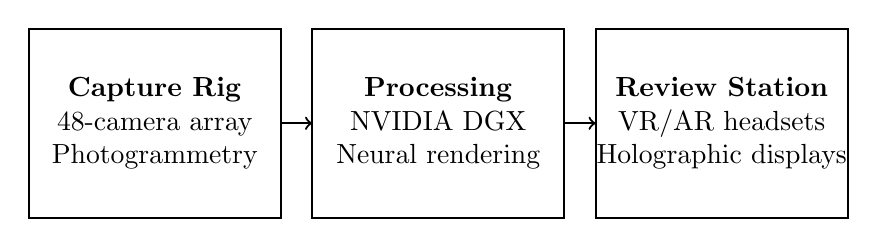
\begin{tikzpicture}[scale=0.8]
    % Capture Area
    \draw[thick] (0,0) rectangle (4,3);
    \node[align=center] at (2,1.5) {\textbf{Capture Rig}\\48-camera array\\Photogrammetry};
    
    % Processing Station
    \draw[thick] (4.5,0) rectangle (8.5,3);
    \node[align=center] at (6.5,1.5) {\textbf{Processing}\\NVIDIA DGX\\Neural rendering};
    
    % Review Area
    \draw[thick] (9,0) rectangle (13,3);
    \node[align=center] at (11,1.5) {\textbf{Review Station}\\VR/AR headsets\\Holographic displays};
    
    % Arrows showing workflow
    \draw[thick,->] (4,1.5) -- (4.5,1.5);
    \draw[thick,->] (8.5,1.5) -- (9,1.5);
\end{tikzpicture}
\end{center}

Equipment includes:
\begin{itemize}
    \item 48-camera photogrammetry array with synchronized capture
    \item NVIDIA DGX A100 for real-time neural rendering
    \item LiDAR scanning equipment (Leica BLK360)
    \item Holographic displays for 3D visualization
    \item Custom software pipeline for gaussian splatting workflows
\end{itemize}

\subsubsection{Telepresence \& XR Laboratory}

\begin{itemize}
    \item Microsoft HoloLens 2 development kits (10 units)
    \item Meta Quest Pro headsets with hand tracking (15 units)
    \item Varjo Aero professional VR headsets (5 units)
    \item Volumetric capture stage with depth cameras
    \item 5G private network for low-latency streaming
    \item Spatial audio system for immersive communication
\end{itemize}

\subsection{Engineering Simulation Visualization Suite}

\subsubsection{Hardware Infrastructure}

\begin{labspec}
Simulation Workstations & Threadripper PRO, RTX 4090, 128GB RAM & 8 & \pounds{64,000} \\
VR/AR Stations & High-end PCs with professional headsets & 6 & \pounds{36,000} \\
Visualization Wall & 4×4 4K display array & 1 & \pounds{25,000} \\
Haptic Devices & Force feedback for CAE interaction & 4 & \pounds{12,000} \\
\end{labspec}

\subsubsection{Software Ecosystem}

\begin{itemize}
    \item Engineering: Ansys, COMSOL, Simulink, SolidWorks
    \item Visualization: Unreal Engine, Unity, ParaView, EnSight
    \item Creative: Houdini, Nuke, DaVinci Resolve, Cinema 4D
    \item AI/ML: TensorFlow, PyTorch, CUDA toolkit, ComfyUI
    \item Collaboration: Perforce, Shotgrid, ftrack, Slack
\end{itemize}

\subsection{Drone Technology Center}

\subsubsection{Flight Training Area}

\begin{itemize}
    \item Indoor netted flight space (15m × 10m × 5m)
    \item Outdoor flight zone with CAA permissions
    \item Weather monitoring station
    \item Charging and maintenance stations
    \item Safety equipment and protocols
\end{itemize}

\subsubsection{Drone Fleet}

\begin{table}[H]
\centering
\begin{tabular}{lll}
\toprule
\textbf{Type} & \textbf{Models} & \textbf{Applications} \\
\midrule
Cinema Drones & DJI Inspire 3, FPV & Aerial cinematography \\
Mapping Drones & DJI M300 RTK, P4 RTK & Photogrammetry, surveying \\
Racing Drones & Custom 5" FPV builds & Pilot training, agility \\
Autonomous & PX4 development platforms & Computer vision, AI navigation \\
\bottomrule
\end{tabular}
\end{table}

\subsection{Supporting Infrastructure}

\subsubsection{Compute and Rendering Farm}

\begin{itemize}
    \item NVIDIA DGX A100 system for AI/ML training
    \item 20-node render farm with RTX 4090 GPUs
    \item 500TB high-speed storage array
    \item 10Gbps internal network with 100Gbps backbone
    \item Cloud burst capability to AWS/Azure
\end{itemize}

\subsubsection{Collaboration Spaces}

\begin{center}
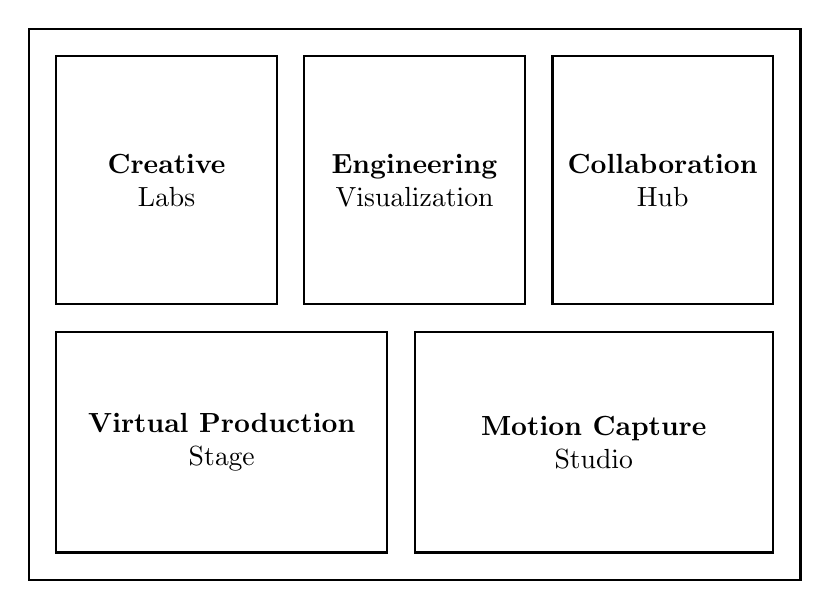
\begin{tikzpicture}[scale=0.7]
    % Main Building Layout
    \draw[thick] (0,0) rectangle (14,10);
    
    % VP Stage
    \draw[thick] (0.5,0.5) rectangle (6.5,4.5);
    \node[align=center] at (3.5,2.5) {\textbf{Virtual Production}\\Stage};
    
    % MoCap Studio
    \draw[thick] (7,0.5) rectangle (13.5,4.5);
    \node[align=center] at (10.25,2.5) {\textbf{Motion Capture}\\Studio};
    
    % Creative Labs
    \draw[thick] (0.5,5) rectangle (4.5,9.5);
    \node[align=center] at (2.5,7.25) {\textbf{Creative}\\Labs};
    
    % Engineering Suite
    \draw[thick] (5,5) rectangle (9,9.5);
    \node[align=center] at (7,7.25) {\textbf{Engineering}\\Visualization};
    
    % Collaboration Hub
    \draw[thick] (9.5,5) rectangle (13.5,9.5);
    \node[align=center] at (11.5,7.25) {\textbf{Collaboration}\\Hub};
\end{tikzpicture}
\end{center}

\subsection{Sustainable Features - Enhanced}

\subsubsection{Renewable Energy System}

\begin{solarroi}
\textbf{18kW Solar Installation with Battery Storage}

\begin{table}[H]
\centering
\begin{tabular}{lr}
\toprule
\textbf{Component} & \textbf{Specification} \\
\midrule
Solar Panels & 45x 400W panels (18kW total) \\
Battery Storage & 4x Tesla Powerwall (54kWh) \\
Annual Generation & 16,500 kWh estimated \\
Tech Load Offset & 60\% of compute/render power \\
Grid Independence & 40-50\% overall average \\
25-year Savings & \pounds{285,000} projected \\
\bottomrule
\end{tabular}
\end{table}
\end{solarroi}

\subsubsection{Sustainable Technology Practices}

\begin{itemize}
    \item GPU power management with workload scheduling
    \item Waste heat recovery for building heating
    \item Rainwater harvesting for cooling systems
    \item LED lighting throughout with motion sensors
    \item EV charging integrated with solar generation
\end{itemize}

\subsection{Accommodation Features - Tech Enhanced}

\subsubsection{Smart Residence Features}

The renovated Welsh farmhouse combines traditional charm with cutting-edge technology:

\begin{itemize}
    \item \textbf{Tech Amenities}: Gigabit WiFi, smart home automation, streaming studio
    \item \textbf{Work Spaces}: Private offices with dual 4K monitors, ergonomic furniture
    \item \textbf{Collaboration}: Video conferencing suite, brainstorming room with digital whiteboards
    \item \textbf{Wellness}: VR meditation room, biophilic design elements
    \item \textbf{Entertainment}: Home theater with Dolby Atmos, gaming lounge
\end{itemize}

\subsection{Accessibility and Inclusivity}

DreamLab is committed to universal design principles:

\begin{itemize}
    \item All facilities wheelchair accessible with automatic doors
    \item Height-adjustable workstations throughout
    \item Assistive technology including eye-tracking interfaces
    \item Sign language interpretation available
    \item Neurodiversity-friendly spaces with adjustable lighting/sound
    \item Gender-neutral facilities
\end{itemize}
\section{House Renovation Plan}
\label{sec:house-renovation}

\subsection{Overview}

This section details the comprehensive renovation plan for Fairfield House in Eskdale Green, Lake District. The renovation encompasses both the residential improvements and the conversion of the right-hand wing into a dual-use executive training facility and holiday let accommodation.

\subsection{Renovation Scope and Costs}

\begin{table}[H]
\centering
\begin{tabularx}{\textwidth}{|l|X|r|r|}
\hline
\textbf{Item} & \textbf{Description} & \textbf{Low Estimate} & \textbf{High Estimate} \\
\hline
Triple Glazed Window & Additional large window, second floor & £1,200 & £1,700 \\
Kitchen Refit & Complete residential kitchen & £15,000 & £25,000 \\
Trim \& Finishes & Making good throughout property & £2,000 & £3,500 \\
Chimney/Fire & Wood burning stove installation & £3,500 & £5,500 \\
Garden Clearing & Clear 0.5 acre & £1,500 & £3,000 \\
Shed/Woodstore & Quality outdoor storage & £2,000 & £4,000 \\
Trampoline Pit & Excavation and installation & £2,500 & £4,000 \\
Solar Pergola x3 & 3 × 10m² structures (6kW) & £22,200 & £22,200 \\
Outdoor Sauna & 6-person panoramic view & £12,160 & £17,160 \\
Battery Storage & Tesla Powerwall 3 & £10,795 & £11,100 \\
Shelving Units & Built-in storage & £2,000 & £3,500 \\
Rabbit Hutch & Weather-resistant & £500 & £1,000 \\
Trifold Doors x2 & 8m wide triple glazed & £25,000 & £40,000 \\
Luxury Shower & Large wetroom refit & £12,000 & £20,000 \\
\hline
\textbf{Subtotal} & & \textbf{£112,355} & \textbf{£161,660} \\
\textbf{With 15\% Contingency} & & \textbf{£129,208} & \textbf{£185,909} \\
\hline
\end{tabularx}
\caption{House Renovation Cost Breakdown}
\label{tab:renovation-costs}
\end{table}

\begin{figure}[H]
    \centering
    \includegraphics[width=0.7\textwidth]{media/winecellar.png}
    \caption{A key feature of the renovation: a modern, climate-controlled wine cellar.}
    \label{fig:wine-cellar}
\end{figure}

\subsection{Implementation Timeline}

The renovation will be executed over 18 months in four distinct phases:

\subsubsection{Phase 1: Essential Structural (Months 1-3)}
\begin{itemize}
    \item Installation of 8m trifold doors (weather-tight priority)
    \item Complete kitchen refit
    \item Triple glazed window installation
    \item \textbf{Budget: £41,200 - £66,700}
\end{itemize}

\subsubsection{Phase 2: Core Improvements (Months 4-9)}
\begin{itemize}
    \item Chimney preparation and wood burning stove
    \item Luxury shower/wetroom conversion
    \item Tesla Powerwall battery system
    \item Interior trim and finishes
    \item \textbf{Budget: £28,295 - £39,600}
\end{itemize}

\subsubsection{Phase 3: External Works (Months 10-15)}
\begin{itemize}
    \item Solar pergola construction (3 × 10m² units)
    \item Garden clearance and landscaping
    \item Shed/woodstore construction
    \item \textbf{Budget: £25,700 - £29,200}
\end{itemize}

\subsubsection{Phase 4: Leisure Items (Months 16-18)}
\begin{itemize}
    \item Outdoor sauna installation
    \item Trampoline pit excavation and fitting
    \item Custom shelving throughout
    \item Rabbit hutch construction
    \item \textbf{Budget: £17,160 - £25,660}
\end{itemize}

\subsection{Solar Pergola System\index{Solar Pergola}}

The solar installation consists of three pergolas, each under 10m² to comply with Lake District National Park permitted development rights:

\begin{itemize}
    \item \textbf{Total Capacity:} 6kW (3 × 2kW)
    \item \textbf{Annual Generation:} Approximately 4,800 kWh
    \item \textbf{Configuration:} 18 × 330W panels total
    \item \textbf{Location:} Within 20m curtilage of main dwelling
    \item \textbf{Grid Connection:} Zero-export configuration
\end{itemize}

\subsection{Integration with Business Operations}

The renovation timeline is carefully coordinated with the business launch:

\begin{enumerate}
    \item \textbf{Q1-Q2 2025:} Essential structural work ensures weather-tight property
    \item \textbf{Q3-Q4 2025:} Core improvements create functional spaces
    \item \textbf{Q1-Q2 2026:} External works and lab fit-out proceed in parallel
    \item \textbf{Q3-Q4 2026:} Final touches and soft launch of training facility
    \item \textbf{Q1 2027:} Full operational launch with integrated systems
\end{enumerate}

\subsection{Planning and Regulatory Compliance}

\begin{itemize}
    \item \textbf{Permitted Development:} Solar pergolas comply with Class E rights
    \item \textbf{Building Control:} Required for trifold doors and major alterations
    \item \textbf{Lake District NP:} All external works designed to meet local guidelines
    \item \textbf{Fire Safety:} Integrated detection system throughout converted areas
\end{itemize}

\subsection{Risk Mitigation}

\begin{itemize}
    \item \textbf{Weather Delays:} Indoor work scheduled for winter months
    \item \textbf{Contractor Availability:} Local contractors pre-booked 3-6 months ahead
    \item \textbf{Material Shortages:} Long-lead items ordered in Phase 1
    \item \textbf{Budget Overruns:} 15\% contingency included in all estimates
    \item \textbf{Family Disruption:} Phased approach maintains livability throughout
\end{itemize}
\section{Business Model \& Revenue Streams}

\subsection{Dual Revenue Model Overview}

DreamLab's innovative business model leverages complementary revenue streams that maximise facility utilisation:

\begin{center}
\begin{tikzpicture}[scale=0.9]
    % Central hub
    \node[circle, draw=dreamlab-purple, fill=dreamlab-lightgrey, minimum size=3cm, align=center] (hub) at (0,0) {
        \textbf{DreamLab}\\
        \textbf{Revenue Hub}
    };
    
    % Training revenue
    \node[rectangle, draw=dreamlab-blue, fill=dreamlab-blue!20, minimum width=4cm, minimum height=2cm, align=center] (training) at (-5,2) {
        \textbf{AI Training}\\
        Mon-Fri Focus\\
        70\% of revenue
    };
    
    % Letting revenue
    \node[rectangle, draw=dreamlab-green, fill=dreamlab-green!20, minimum width=4cm, minimum height=2cm, align=center] (letting) at (5,2) {
        \textbf{Holiday Letting}\\
        Weekends/Holidays\\
        20\% of revenue
    };
    
    % Consultancy revenue
    \node[rectangle, draw=dreamlab-orange, fill=dreamlab-orange!20, minimum width=4cm, minimum height=2cm, align=center] (consult) at (-5,-2) {
        \textbf{Consultancy}\\
        Project-based\\
        10\% of revenue
    };
    
    % Online revenue
    \node[rectangle, draw=dreamlab-grey, fill=dreamlab-grey!20, minimum width=4cm, minimum height=2cm, align=center] (online) at (5,-2) {
        \textbf{Online/Hybrid}\\
        Scalable growth\\
        Future expansion
    };
    
    % Connections
    \draw[thick, ->] (training) -- (hub);
    \draw[thick, ->] (letting) -- (hub);
    \draw[thick, ->] (consult) -- (hub);
    \draw[thick, ->] (online) -- (hub);
\end{tikzpicture}
\end{center}

\subsection{Revenue Stream Analysis}

\subsubsection{Training Revenue (Primary)}

\begin{table}[H]
\centering
\begin{tabularx}{\textwidth}{lrrrrr}
\toprule
\textbf{Training Type} & \textbf{Price/Person} & \textbf{Capacity} & \textbf{Frequency} & \textbf{Annual Sessions} & \textbf{Revenue} \\
\midrule
3-Day Bootcamp & \pounds{1,495} & 12 & Weekly & 40 & \pounds{718,000} \\
2-Day Workshop & \pounds{995} & 12 & Bi-weekly & 20 & \pounds{238,000} \\
5-Day Intensive & \pounds{2,995} & 10 & Monthly & 10 & \pounds{299,000} \\
Corporate Package & \pounds{25,000} & Team & Monthly & 12 & \pounds{300,000} \\
\midrule
\multicolumn{5}{r}{\textbf{Total Training Revenue (Year 3):}} & \textbf{\pounds{1,555,000}} \\
\bottomrule
\end{tabularx}
\end{table}

\subsubsection{Holiday Let Revenue (Secondary)}

\begin{table}[H]
\centering
\begin{tabular}{lrrrr}
\toprule
\textbf{Season} & \textbf{Nightly Rate} & \textbf{Occupancy} & \textbf{Available Nights} & \textbf{Revenue} \\
\midrule
Peak (Jul-Aug) & \pounds{350} & 90\% & 60 & \pounds{18,900} \\
High (Apr-Jun, Sep-Oct) & \pounds{250} & 75\% & 120 & \pounds{22,500} \\
Low (Nov-Mar) & \pounds{175} & 40\% & 100 & \pounds{7,000} \\
\midrule
\multicolumn{4}{r}{\textbf{Total Annual Letting Revenue:}} & \textbf{\pounds{48,400}} \\
\bottomrule
\end{tabular}
\end{table}

\subsection{Customer Acquisition Strategy}

\subsubsection{B2B Sales Process}

\begin{enumerate}
    \item \textbf{Lead Generation}
    \begin{itemize}
        \item LinkedIn outreach to L\&D managers
        \item Tech Wales network events
        \item Webinar series on AI adoption
        \item Partnership referrals
    \end{itemize}
    
    \item \textbf{Sales Funnel}
    \begin{itemize}
        \item Initial consultation (free)
        \item Facility tour (virtual/in-person)
        \item Customised proposal
        \item Pilot programme option
        \item Contract negotiation
    \end{itemize}
    
    \item \textbf{Account Management}
    \begin{itemize}
        \item Dedicated account manager
        \item Quarterly business reviews
        \item Continuous curriculum updates
        \item Alumni network access
    \end{itemize}
\end{enumerate}

\subsubsection{B2C Marketing Channels}

\begin{table}[H]
\centering
\begin{tabularx}{\textwidth}{lXrr}
\toprule
\textbf{Channel} & \textbf{Strategy} & \textbf{Budget} & \textbf{Expected ROI} \\
\midrule
Google Ads & Targeted keywords: "AI training UK" & \pounds{2,000}/mo & 3.5x \\
LinkedIn Ads & Professional targeting & \pounds{1,500}/mo & 4.2x \\
Content Marketing & Blog, tutorials, case studies & \pounds{1,000}/mo & 5.8x \\
Email Marketing & Nurture campaigns & \pounds{500}/mo & 8.3x \\
Airbnb/Booking & Holiday let promotion & 15\% commission & 6.5x \\
\bottomrule
\end{tabularx}
\end{table}

\subsection{Pricing Strategy}

\subsubsection{Value-Based Pricing Model}

Our pricing reflects the unique value proposition:

\begin{keypoint}
\textbf{Premium Positioning Justified By:}
\begin{itemize}
    \item Exclusive access to DGX A100 system (£150k equipment)
    \item Small class sizes (max 12) ensuring individual attention
    \item Accommodation included reducing total trip cost
    \item Industry expert instructors with practical experience
    \item Post-training support and alumni network
\end{itemize}
\end{keypoint}

\subsubsection{Dynamic Pricing Elements}

\begin{itemize}
    \item \textbf{Early Bird Discounts}: 15\% off for bookings 2+ months ahead
    \item \textbf{Group Rates}: 20\% discount for 5+ participants
    \item \textbf{Alumni Pricing}: 25\% off returning students
    \item \textbf{Off-Peak Rates}: 30\% reduction for November-February training
    \item \textbf{Welsh Business Discount}: 10\% for local companies
\end{itemize}

\subsection{Customer Retention Strategy}

\begin{center}
\begin{tikzpicture}[node distance=2.5cm]
    \node[rectangle, draw=dreamlab-purple, fill=dreamlab-purple!20, align=center] (acquire) {
        \textbf{Acquire}\\
        First training\\
        experience
    };
    
    \node[rectangle, draw=dreamlab-blue, fill=dreamlab-blue!20, align=center, right=of acquire] (engage) {
        \textbf{Engage}\\
        Alumni network\\
        Continuous learning
    };
    
    \node[rectangle, draw=dreamlab-green, fill=dreamlab-green!20, align=center, right=of engage] (expand) {
        \textbf{Expand}\\
        Advanced courses\\
        Team training
    };
    
    \node[rectangle, draw=dreamlab-orange, fill=dreamlab-orange!20, align=center, below=of engage] (advocate) {
        \textbf{Advocate}\\
        Referrals\\
        Case studies
    };
    
    \draw[thick, ->] (acquire) -- (engage);
    \draw[thick, ->] (engage) -- (expand);
    \draw[thick, ->] (expand) -- (advocate);
    \draw[thick, ->] (advocate) -- (acquire);
\end{tikzpicture}
\end{center}

\subsection{Partnership Revenue Model}

Strategic partnerships provide additional revenue streams:

\begin{itemize}
    \item \textbf{University Partnerships}: \pounds{50,000}/year for student programmes
    \item \textbf{Vendor Certifications}: 20\% commission on certification exams
    \item \textbf{Corporate Memberships}: \pounds{25,000}/year for unlimited access
    \item \textbf{Government Contracts}: Welsh Gov skills programmes
\end{itemize}

\subsection{Unit Economics}

\begin{table}[H]
\centering
\begin{tabular}{lrr}
\toprule
\textbf{Metric} & \textbf{Training} & \textbf{Holiday Let} \\
\midrule
Average Transaction Value & \pounds{1,745} & \pounds{185}/night \\
Customer Acquisition Cost & \pounds{215} & \pounds{45} \\
Gross Margin & 68\% & 82\% \\
Customer Lifetime Value & \pounds{8,500} & \pounds{1,200} \\
Payback Period & 1.2 months & 0.8 months \\
\bottomrule
\end{tabular}
\end{table}
\section{Financial Projections}

\subsection{Revenue Model Overview}

DreamLab's diversified revenue model capitalizes on multiple high-growth markets while maintaining stable base revenue from established sectors.

\subsubsection{Revenue Stream Breakdown}

\begin{table}
\centering
\begin{tabular}{lrrrrr}
\toprule
\textbf{Revenue Stream} & \textbf{Year 1} & \textbf{Year 2} & \textbf{Year 3} & \textbf{Year 4} & \textbf{Year 5} \\
\midrule
\multicolumn{6}{l}{\textit{Training Programs}} \\
Creative Technology & \pounds{173,000} & \pounds{520,000} & \pounds{1,225,000} & \pounds{1,820,000} & \pounds{2,275,000} \\
Agentic Engineering & \pounds{124,000} & \pounds{372,000} & \pounds{875,000} & \pounds{1,300,000} & \pounds{1,625,000} \\
Engineering Simulation & \pounds{99,000} & \pounds{297,000} & \pounds{700,000} & \pounds{910,000} & \pounds{1,170,000} \\
Nuclear \& Energy & \pounds{74,000} & \pounds{223,000} & \pounds{525,000} & \pounds{630,000} & \pounds{780,000} \\
\midrule
\multicolumn{6}{l}{\textit{Other Revenue}} \\
Equipment Rental & \pounds{15,000} & \pounds{60,000} & \pounds{150,000} & \pounds{225,000} & \pounds{300,000} \\
Online Programs & \pounds{10,000} & \pounds{40,000} & \pounds{125,000} & \pounds{250,000} & \pounds{400,000} \\
Consulting & \pounds{0} & \pounds{50,000} & \pounds{150,000} & \pounds{250,000} & \pounds{350,000} \\
Accommodation & \pounds{45,000} & \pounds{90,000} & \pounds{150,000} & \pounds{180,000} & \pounds{200,000} \\
\midrule
\textbf{Total Revenue} & \textbf{\pounds{540,000}} & \textbf{\pounds{1,652,000}} & \textbf{\pounds{3,900,000}} & \textbf{\pounds{5,565,000}} & \textbf{\pounds{7,100,000}} \\
\bottomrule
\end{tabular}
\end{table}

\subsection{Student Volume Projections}

\begin{table}
\centering
\begin{tabular}{lrrrrr}
\toprule
\textbf{Program Category} & \textbf{Year 1} & \textbf{Year 2} & \textbf{Year 3} & \textbf{Year 4} & \textbf{Year 5} \\
\midrule
Creative Technology & 40 & 120 & 250 & 350 & 425 \\
Agentic Engineering & 35 & 105 & 220 & 310 & 375 \\
Engineering Simulation & 30 & 90 & 175 & 210 & 260 \\
Nuclear \& Energy & 20 & 60 & 125 & 150 & 180 \\
Online Learners & 50 & 200 & 500 & 1,000 & 1,600 \\
\midrule
\textbf{Total Students} & \textbf{175} & \textbf{575} & \textbf{1,270} & \textbf{2,020} & \textbf{2,840} \\
\bottomrule
\end{tabular}
\end{table}

\subsection{Operating Expenses}

\begin{table}
\centering
\begin{tabular}{lrrrrr}
\toprule
\textbf{Expense Category} & \textbf{Year 1} & \textbf{Year 2} & \textbf{Year 3} & \textbf{Year 4} & \textbf{Year 5} \\
\midrule
\multicolumn{6}{l}{\textit{Staff Costs}} \\
Core Team (4 FTE) & \pounds{300,000} & \pounds{350,000} & \pounds{400,000} & \pounds{450,000} & \pounds{500,000} \\
Instructors & \pounds{60,000} & \pounds{180,000} & \pounds{420,000} & \pounds{600,000} & \pounds{750,000} \\
Support Staff & \pounds{40,000} & \pounds{80,000} & \pounds{120,000} & \pounds{160,000} & \pounds{200,000} \\
\midrule
\multicolumn{6}{l}{\textit{Facility Costs}} \\
Lease/Mortgage & \pounds{96,000} & \pounds{96,000} & \pounds{96,000} & \pounds{96,000} & \pounds{96,000} \\
Utilities & \pounds{30,000} & \pounds{36,000} & \pounds{42,000} & \pounds{48,000} & \pounds{54,000} \\
Maintenance & \pounds{15,000} & \pounds{20,000} & \pounds{25,000} & \pounds{30,000} & \pounds{35,000} \\
Insurance & \pounds{25,000} & \pounds{30,000} & \pounds{35,000} & \pounds{40,000} & \pounds{45,000} \\
\midrule
\multicolumn{6}{l}{\textit{Technology \& Equipment}} \\
Equipment Lease & \pounds{144,000} & \pounds{144,000} & \pounds{144,000} & \pounds{144,000} & \pounds{144,000} \\
Software Licenses & \pounds{50,000} & \pounds{75,000} & \pounds{100,000} & \pounds{125,000} & \pounds{150,000} \\
Tech Refresh & \pounds{0} & \pounds{50,000} & \pounds{100,000} & \pounds{150,000} & \pounds{200,000} \\
\midrule
\multicolumn{6}{l}{\textit{Marketing \& Sales}} \\
Digital Marketing & \pounds{30,000} & \pounds{60,000} & \pounds{90,000} & \pounds{120,000} & \pounds{150,000} \\
Events \& Conferences & \pounds{20,000} & \pounds{40,000} & \pounds{60,000} & \pounds{80,000} & \pounds{100,000} \\
Sales Team & \pounds{0} & \pounds{60,000} & \pounds{120,000} & \pounds{180,000} & \pounds{240,000} \\
\midrule
\multicolumn{6}{l}{\textit{Other Operating}} \\
Materials \& Supplies & \pounds{15,000} & \pounds{45,000} & \pounds{100,000} & \pounds{150,000} & \pounds{200,000} \\
Professional Services & \pounds{20,000} & \pounds{30,000} & \pounds{40,000} & \pounds{50,000} & \pounds{60,000} \\
Miscellaneous & \pounds{10,000} & \pounds{20,000} & \pounds{30,000} & \pounds{40,000} & \pounds{50,000} \\
\midrule
\textbf{Total Expenses} & \textbf{\pounds{855,000}} & \textbf{\pounds{1,370,000}} & \textbf{\pounds{1,922,000}} & \textbf{\pounds{2,513,000}} & \textbf{\pounds{3,129,000}} \\
\bottomrule
\end{tabular}
\end{table}

\subsection{Profitability Analysis}

\begin{table}
\centering
\begin{tabular}{lrrrrr}
\toprule
\textbf{Metric} & \textbf{Year 1} & \textbf{Year 2} & \textbf{Year 3} & \textbf{Year 4} & \textbf{Year 5} \\
\midrule
Revenue & \pounds{540,000} & \pounds{1,652,000} & \pounds{3,900,000} & \pounds{5,565,000} & \pounds{7,100,000} \\
Operating Expenses & \pounds{855,000} & \pounds{1,370,000} & \pounds{1,922,000} & \pounds{2,513,000} & \pounds{3,129,000} \\
\midrule
EBITDA & (\pounds{315,000}) & \pounds{282,000} & \pounds{1,978,000} & \pounds{3,052,000} & \pounds{3,971,000} \\
EBITDA Margin & -58\% & 17\% & 51\% & 55\% & 56\% \\
\midrule
Depreciation & \pounds{120,000} & \pounds{140,000} & \pounds{160,000} & \pounds{180,000} & \pounds{200,000} \\
Interest & \pounds{45,000} & \pounds{40,000} & \pounds{35,000} & \pounds{30,000} & \pounds{25,000} \\
\midrule
Net Income & (\pounds{480,000}) & \pounds{102,000} & \pounds{1,783,000} & \pounds{2,842,000} & \pounds{3,746,000} \\
Net Margin & -89\% & 6\% & 46\% & 51\% & 53\% \\
\bottomrule
\end{tabular}
\end{table}

\subsection{Cash Flow Projections}

% Commenting out pgfplots chart due to "Dimension too large" error
% \begin{figure}
% \centering
% \begin{tikzpicture}
% \begin{axis}[
%     title={5-Year Cash Flow Projection},
%     xlabel={Year},
%     ylabel={Cash Flow (\pounds)},
%     xmin=0.5, xmax=5.5,
%     ymin=-1000000, ymax=4000000,
%     xtick={1,2,3,4,5},
%     scaled ticks=false,
%     yticklabel={\pgfmathparse{\tick/1000000}\pgfmathprintnumber{\pgfmathresult}M},
%     legend pos=north west,
%     ymajorgrids=true,
%     grid style=dashed,
%     width=\textwidth,
%     height=8cm,
% ]
%
% \addplot[
%     color=dreamlab-blue,
%     mark=square*,
%     line width=2pt
% ]
% coordinates {
%     (1,-480000)
%     (2,102000)
%     (3,1783000)
%     (4,2842000)
%     (5,3746000)
% };
% \addlegendentry{Net Income}
%
% \addplot[
%     color=dreamlab-green,
%     mark=*,
%     line width=2pt
% ]
% coordinates {
%     (1,-480000)
%     (2,-378000)
%     (3,1405000)
%     (4,4247000)
%     (5,7993000)
% };
% \addlegendentry{Cumulative Cash}
%
% \end{axis}
% \end{tikzpicture}
% \end{figure}

\begin{table}
\centering
\begin{tabular}{lrrrrr}
\toprule
\textbf{Year} & \textbf{Net Income} & \textbf{Depreciation} & \textbf{CapEx} & \textbf{Working Capital} & \textbf{Free Cash Flow} \\
\midrule
Year 1 & (\pounds{480,000}) & \pounds{120,000} & (\pounds{700,000}) & (\pounds{50,000}) & (\pounds{1,110,000}) \\
Year 2 & \pounds{102,000} & \pounds{140,000} & (\pounds{150,000}) & (\pounds{30,000}) & \pounds{62,000} \\
Year 3 & \pounds{1,783,000} & \pounds{160,000} & (\pounds{100,000}) & (\pounds{40,000}) & \pounds{1,803,000} \\
Year 4 & \pounds{2,842,000} & \pounds{180,000} & (\pounds{150,000}) & (\pounds{30,000}) & \pounds{2,842,000} \\
Year 5 & \pounds{3,746,000} & \pounds{200,000} & (\pounds{200,000}) & (\pounds{20,000}) & \pounds{3,726,000} \\
\midrule
\textbf{Cumulative} & \textbf{\pounds{7,993,000}} & & & & \textbf{\pounds{7,323,000}} \\
\bottomrule
\end{tabular}
\end{table}

\subsection{Investment Requirements \& Use of Funds}

\subsubsection{Total Investment: \pounds{950,000}}

\begin{table}
\centering
\begin{tabular}{lrr}
\toprule
\textbf{Investment Category} & \textbf{Amount} & \textbf{\% of Total} \\
\midrule
\multicolumn{3}{l}{\textit{Technology Infrastructure}} \\
Virtual Production Equipment & \pounds{350,000} & 37\% \\
Agentic Engineering Lab & \pounds{200,000} & 21\% \\
Computing \& Simulation & \pounds{200,000} & 21\% \\
\midrule
\multicolumn{3}{l}{\textit{Facility Development}} \\
Building Renovation & \pounds{100,000} & 11\% \\
Sustainable Energy Systems & \pounds{50,000} & 5\% \\
\midrule
Working Capital & \pounds{50,000} & 5\% \\
\midrule
\textbf{Total Investment} & \textbf{\pounds{950,000}} & \textbf{100\%} \\
\bottomrule
\end{tabular}
\end{table}

\subsection{Return on Investment}

\begin{keypoint}
\textbf{Investment Returns Analysis}
\begin{itemize}
    \item \textbf{Payback Period}: 2.8 years
    \item \textbf{Internal Rate of Return (IRR)}: 52\% over 5 years
    \item \textbf{Net Present Value (NPV)}: \pounds{4.2M at 12\% discount rate}
    \item \textbf{Return on Investment (ROI)}: 740\% by Year 5
\end{itemize}
\end{keypoint}

\subsection{Sensitivity Analysis}

\begin{table}
\centering
\begin{tabular}{lrrr}
\toprule
\textbf{Scenario} & \textbf{Revenue Impact} & \textbf{Year 3 EBITDA} & \textbf{5-Year NPV} \\
\midrule
Base Case & 100\% & \pounds{1,978,000} & \pounds{4,200,000} \\
Optimistic (+20\%) & 120\% & \pounds{2,420,000} & \pounds{5,500,000} \\
Conservative (-20\%) & 80\% & \pounds{1,536,000} & \pounds{2,900,000} \\
Worst Case (-40\%) & 60\% & \pounds{1,094,000} & \pounds{1,600,000} \\
\bottomrule
\end{tabular}
\end{table}

\subsection{Key Financial Metrics}

\begin{table}
\centering
\begin{tabular}{lrrrrr}
\toprule
\textbf{Metric} & \textbf{Year 1} & \textbf{Year 2} & \textbf{Year 3} & \textbf{Year 4} & \textbf{Year 5} \\
\midrule
Gross Margin & 42\% & 58\% & 72\% & 75\% & 77\% \\
Operating Margin & -58\% & 17\% & 51\% & 55\% & 56\% \\
Current Ratio & 0.8 & 1.2 & 2.5 & 3.8 & 5.2 \\
Revenue per Student & \pounds{3,086} & \pounds{2,873} & \pounds{3,071} & \pounds{2,755} & \pounds{2,500} \\
Customer Acquisition Cost & \pounds{343} & \pounds{278} & \pounds{189} & \pounds{149} & \pounds{123} \\
\bottomrule
\end{tabular}
\end{table}
\section{Implementation Timeline}

\subsection{Phased Development Approach}

DreamLab's implementation follows a strategic phased approach, prioritizing revenue-generating capabilities while building toward full operational capacity.

\subsection{Phase 1: Foundation (Months 1-3)}

\subsubsection{Key Objectives}
\begin{itemize}
    \item Secure facility and initial funding
    \item Core team recruitment
    \item Essential equipment procurement
    \item Initial program development
    \item Marketing launch preparation
\end{itemize}

\subsubsection{Detailed Timeline}

\begin{center}
\begin{ganttchart}[
    hgrid,
    vgrid,
    x unit=0.8cm,
    y unit title=0.6cm,
    y unit chart=0.5cm,
    title label font=\footnotesize,
    bar label font=\footnotesize,
    group label font=\footnotesize\bfseries,
    milestone label font=\footnotesize\itshape
]{1}{12}
    \gantttitle{Year 1}{12} \\
    \gantttitlelist{1,...,12}{1} \\
    \ganttgroup{Phase 1: Foundation}{1}{3} \\
    \ganttbar{Facility Setup}{1}{2} \\
    \ganttbar{Team Recruitment}{1}{2} \\
    \ganttbar{Equipment Order}{2}{3} \\
    \ganttmilestone{Facility Ready}{3} \\
    \ganttgroup{Phase 2: Launch}{4}{6} \\
    \ganttbar{Equipment Install}{4}{5} \\
    \ganttbar{Program Development}{3}{5} \\
    \ganttbar{Marketing Campaign}{4}{6} \\
    \ganttmilestone{First Course}{6} \\
    \ganttgroup{Phase 3: Growth}{7}{9} \\
    \ganttbar{Course Expansion}{7}{9} \\
    \ganttbar{Partnership Building}{6}{9} \\
    \ganttbar{Online Platform}{7}{9} \\
    \ganttmilestone{Full Operations}{9} \\
    \ganttgroup{Phase 4: Scale}{10}{12} \\
    \ganttbar{Advanced Programs}{10}{12} \\
    \ganttbar{Corporate Training}{10}{12} \\
    \ganttbar{Certification Launch}{11}{12} \\
    \ganttmilestone{Year 1 Complete}{12}
\end{ganttchart}
\end{center}

\subsection{Phase 2: Launch (Months 4-6)}

\subsubsection{Critical Milestones}
\begin{table}[H]
\centering
\begin{tabularx}{\textwidth}{lXl}
\toprule
\textbf{Milestone} & \textbf{Success Criteria} & \textbf{Target Date} \\
\midrule
Equipment Operational & LED volume calibrated, all systems tested & Month 5 \\
First Program Ready & Virtual Production Masterclass curriculum complete & Month 5 \\
10 Students Enrolled & Initial cohort confirmed with deposits & Month 6 \\
Marketing Live & Website, social media, PR campaign active & Month 4 \\
Partnerships Signed & 2+ technology vendor agreements & Month 6 \\
\bottomrule
\end{tabularx}
\end{table}

\subsection{Phase 3: Growth (Months 7-9)}

\subsubsection{Expansion Activities}
\begin{itemize}
    \item Launch agentic engineering programs
    \item Introduce gaussian splatting workshops
    \item Develop corporate partnerships
    \item Implement online learning platform
    \item Hire additional instructors
\end{itemize}

\subsection{Phase 4: Scale (Months 10-12)}

\subsubsection{Scaling Objectives}
\begin{enumerate}
    \item Achieve 75\% facility utilization
    \item Launch certification programs
    \item Establish international partnerships
    \item Generate first profit
    \item Plan Year 2 expansion
\end{enumerate}

\subsection{Resource Allocation Timeline}

\begin{table}[H]
\centering
\begin{tabular}{lrrrr}
\toprule
\textbf{Resource} & \textbf{Q1} & \textbf{Q2} & \textbf{Q3} & \textbf{Q4} \\
\midrule
\multicolumn{5}{l}{\textit{Human Resources (FTE)}} \\
Core Team & 4 & 6 & 8 & 10 \\
Instructors & 0 & 2 & 4 & 6 \\
Support Staff & 1 & 2 & 3 & 4 \\
\midrule
\multicolumn{5}{l}{\textit{Financial Investment (\pounds{000s})}} \\
Equipment & 200 & 350 & 100 & 50 \\
Marketing & 20 & 40 & 30 & 20 \\
Operations & 50 & 60 & 70 & 80 \\
Working Capital & 30 & 20 & 0 & 0 \\
\midrule
\textbf{Total Quarterly} & \textbf{300} & \textbf{470} & \textbf{200} & \textbf{150} \\
\bottomrule
\end{tabular}
\end{table}

\subsection{Technology Implementation Schedule}

\begin{center}
\begin{tikzpicture}[scale=0.8]
    % Timeline base
    \draw[thick] (0,0) -- (12,0);
    
    % Month markers
    \foreach \x in {0,3,6,9,12}
        \draw (\x,0) -- (\x,-0.2) node[below] {M\x};
    
    % Technology implementations
    \node[rectangle, draw=dreamlab-purple, fill=dreamlab-purple!20, above=0.5cm of 2,0] {LED Volume};
    \draw[thick, dreamlab-purple] (1,0.5) -- (3,0.5);
    
    \node[rectangle, draw=dreamlab-blue, fill=dreamlab-blue!20, above=1.5cm of 3,0] {MoCap Studio};
    \draw[thick, dreamlab-blue] (2,1.5) -- (4,1.5);
    
    \node[rectangle, draw=dreamlab-green, fill=dreamlab-green!20, above=2.5cm of 4,0] {Agentic Lab};
    \draw[thick, dreamlab-green] (3,2.5) -- (5,2.5);
    
    \node[rectangle, draw=dreamlab-orange, fill=dreamlab-orange!20, above=0.5cm of 7,0] {Gaussian Rig};
    \draw[thick, dreamlab-orange] (6,0.5) -- (8,0.5);
    
    \node[rectangle, draw=dreamlab-grey, fill=dreamlab-grey!20, above=1.5cm of 9,0] {Online Platform};
    \draw[thick, dreamlab-grey] (8,1.5) -- (10,1.5);
\end{tikzpicture}
\end{center}

\subsection{Marketing and Sales Timeline}

\subsubsection{Pre-Launch (Months 1-3)}
\begin{itemize}
    \item Brand development and messaging
    \item Website design and development
    \item Content creation pipeline
    \item Industry outreach and networking
    \item Early bird campaign preparation
\end{itemize}

\subsubsection{Launch (Months 4-6)}
\begin{itemize}
    \item Press release and media coverage
    \item Social media campaign activation
    \item Industry event participation
    \item First student testimonials
    \item Partnership announcements
\end{itemize}

\subsection{Critical Success Factors by Phase}

\begin{table}[H]
\centering
\begin{tabularx}{\textwidth}{lXr}
\toprule
\textbf{Phase} & \textbf{Critical Success Factors} & \textbf{Target KPI} \\
\midrule
Foundation & Secure funding, hire core team, facility ready & 100\% complete \\
Launch & First programs delivered, positive feedback & NPS 70+ \\
Growth & Multiple programs running, partnerships active & 50 students \\
Scale & Profitable operations, market recognition & \pounds{150K} revenue \\
\bottomrule
\end{tabularx}
\end{table}

\subsection{Risk Mitigation Timeline}

\begin{itemize}
    \item \textbf{Month 1}: Insurance policies in place
    \item \textbf{Month 2}: Legal structure finalized
    \item \textbf{Month 3}: Compliance certifications initiated
    \item \textbf{Month 6}: First safety audit completed
    \item \textbf{Month 9}: Business continuity plan tested
    \item \textbf{Month 12}: Full risk assessment review
\end{itemize}

\subsection{Year 2-5 Strategic Milestones}

\subsubsection{Year 2: Expansion}
\begin{itemize}
    \item Launch 10 new specialized programs
    \item Achieve 300 students trained
    \item Establish European partnerships
    \item Generate \pounds{1.65M} revenue
    \item Consider Series A funding
\end{itemize}

\subsubsection{Year 3: Market Leadership}
\begin{itemize}
    \item Recognized as UK leader in creative tech training
    \item 650 students across all programs
    \item International online presence
    \item \pounds{3.9M} revenue achieved
    \item Second location evaluation
\end{itemize}

\subsubsection{Year 4: Diversification}
\begin{itemize}
    \item Launch consulting division
    \item Develop proprietary certifications
    \item Strategic acquisitions considered
    \item \pounds{5.5M} revenue target
    \item Exit strategy preparation
\end{itemize}

\subsubsection{Year 5: Exit Readiness}
\begin{itemize}
    \item Achieve \pounds{7.1M} revenue
    \item EBITDA margin exceeds 50\%
    \item Clear market leadership position
    \item Multiple exit options available
    \item Target valuation \pounds{45-65M}
\end{itemize}

\subsection{Implementation Governance}

\begin{keypoint}
\textbf{Governance Structure}
\begin{itemize}
    \item Weekly executive team meetings
    \item Monthly board updates
    \item Quarterly investor reports
    \item Annual strategic planning sessions
    \item Continuous KPI monitoring dashboard
\end{itemize}
\end{keypoint}
\section{Marketing Strategy}

\subsection{Target Market Segmentation}

\subsubsection{Primary Markets}

\begin{table}[H]
\centering
\begin{tabularx}{\textwidth}{lXrr}
\toprule
\textbf{Segment} & \textbf{Description} & \textbf{Size (UK)} & \textbf{Priority} \\
\midrule
Creative Studios & Film, VFX, game development companies & 4,600+ & High \\
Tech Innovators & Companies adopting agentic systems & 2,200+ & High \\
Energy Sector & Nuclear and renewable energy & 1,100+ & High \\
Engineering Firms & CAE/simulation users & 8,400+ & Medium \\
Individual Professionals & Freelancers and career changers & 45,000+ & Low \\
\bottomrule
\end{tabularx}
\end{table}

\subsection{Brand Positioning}

\begin{keypoint}
\textbf{Core Positioning Statement}

"DreamLab is where visionary professionals master tomorrow's technologies today. We're the only residential training facility combining virtual production, agentic engineering, and advanced simulation in an immersive learning environment."

\textbf{Key Differentiators}:
\begin{itemize}
    \item Hands-on access to £2.5M of cutting-edge equipment
    \item Industry leaders as instructors
    \item Residential immersion for accelerated learning
    \item Cross-disciplinary innovation
\end{itemize}
\end{keypoint}

\subsection{Marketing Mix Strategy}

\subsubsection{Product Strategy}
\begin{itemize}
    \item Premium training programs with certification
    \item Continuous curriculum updates based on industry needs
    \item Hybrid online/on-site options for accessibility
    \item Custom corporate programs
\end{itemize}

\subsubsection{Pricing Strategy}
\begin{itemize}
    \item Premium pricing justified by unique value
    \item Early bird discounts (15\%)
    \item Corporate volume discounts (20\%)
    \item Alumni loyalty pricing (25\%)
    \item Government funding assistance
\end{itemize}

\subsubsection{Place Strategy}
\begin{itemize}
    \item Primary facility in Cumbria
    \item Online platform for global reach
    \item Partner locations for satellite programs
    \item On-site corporate training options
\end{itemize}

\subsubsection{Promotion Strategy}
\begin{itemize}
    \item Content marketing leadership
    \item Industry conference presence
    \item Strategic partnerships
    \item Alumni ambassador program
\end{itemize}

\subsection{Digital Marketing Channels}

\begin{table}[H]
\centering
\begin{tabular}{lrrr}
\toprule
\textbf{Channel} & \textbf{Monthly Budget} & \textbf{Target CPA} & \textbf{Expected ROI} \\
\midrule
Google Ads & \pounds{3,000} & \pounds{150} & 4.2x \\
LinkedIn Ads & \pounds{2,500} & \pounds{200} & 3.8x \\
YouTube Pre-roll & \pounds{1,500} & \pounds{175} & 3.5x \\
Facebook/Instagram & \pounds{1,000} & \pounds{125} & 4.5x \\
Industry Publications & \pounds{2,000} & \pounds{250} & 3.0x \\
\bottomrule
\end{tabular}
\end{table}

\subsection{Content Marketing Strategy}

\subsubsection{Content Pillars}
\begin{enumerate}
    \item \textbf{Technical Tutorials}: Weekly deep-dives into emerging tech
    \item \textbf{Industry Insights}: Thought leadership on future trends
    \item \textbf{Success Stories}: Alumni and corporate case studies
    \item \textbf{Behind the Scenes}: Facility tours and instructor profiles
    \item \textbf{Live Demonstrations}: Monthly webinars and workshops
\end{enumerate}

\subsubsection{Content Calendar}
\begin{itemize}
    \item Blog posts: 2-3 per week
    \item YouTube videos: Weekly uploads
    \item Podcast: Bi-weekly episodes
    \item Webinars: Monthly
    \item Email newsletter: Weekly
\end{itemize}

\subsection{Partnership Marketing}

\begin{table}[H]
\centering
\begin{tabularx}{\textwidth}{lXl}
\toprule
\textbf{Partner Type} & \textbf{Value Proposition} & \textbf{Status} \\
\midrule
Technology Vendors & Co-marketing, equipment access & In Progress \\
Industry Bodies & Credibility, member benefits & Planned \\
Universities & Academic pathways, research & Exploratory \\
Government & Funding, regional development & Planned \\
Media Partners & Coverage, thought leadership & Developing \\
\bottomrule
\end{tabularx}
\end{table}

\subsection{Customer Journey Optimization}

\begin{center}
\begin{tikzpicture}[node distance=2.5cm]
    \node[rectangle, draw=dreamlab-purple, fill=dreamlab-purple!20, align=center] (aware) {
        \textbf{Awareness}\\
        SEO, Ads, Content\\
        Partners, PR
    };

    \node[rectangle, draw=dreamlab-blue, fill=dreamlab-blue!20, align=center, right=of aware] (consider) {
        \textbf{Consideration}\\
        Website, Demos\\
        Reviews, Tours
    };

    \node[rectangle, draw=dreamlab-green, fill=dreamlab-green!20, align=center, right=of consider] (decide) {
        \textbf{Decision}\\
        Consultation\\
        Financing, Booking
    };

    \node[rectangle, draw=dreamlab-orange, fill=dreamlab-orange!20, align=center, below=of consider] (loyalty) {
        \textbf{Loyalty}\\
        Alumni Network\\
        Advanced Programs
    };

    \draw[thick, ->] (aware) -- (consider);
    \draw[thick, ->] (consider) -- (decide);
    \draw[thick, ->] (decide) -- (loyalty);
    \draw[thick, ->] (loyalty) -- (aware);
\end{tikzpicture}
\end{center}

\subsection{Launch Campaign Strategy}

\subsubsection{Phase 1: Pre-Launch (Months 1-2)}
\begin{itemize}
    \item Build anticipation with teaser content
    \item Secure industry endorsements
    \item Early bird program announcements
    \item Press embargo preparation
\end{itemize}

\subsubsection{Phase 2: Launch (Month 3)}
\begin{itemize}
    \item Press release to major publications
    \item Virtual facility tour launch
    \item Founding member program
    \item Industry event presence
\end{itemize}

\subsubsection{Phase 3: Growth (Months 4-12)}
\begin{itemize}
    \item Case study development
    \item Referral program activation
    \item Content marketing acceleration
    \item Partnership announcements
\end{itemize}

\subsection{Marketing Metrics \& KPIs}

\begin{table}[H]
\centering
\begin{tabular}{lrr}
\toprule
\textbf{Metric} & \textbf{Target Year 1} & \textbf{Target Year 3} \\
\midrule
Website Traffic & 10,000/month & 50,000/month \\
Conversion Rate & 2\% & 4\% \\
Cost per Acquisition & \pounds{200} & \pounds{150} \\
Email Subscribers & 5,000 & 25,000 \\
Social Media Followers & 10,000 & 50,000 \\
PR Mentions & 50 & 200 \\
NPS Score & 70+ & 80+ \\
\bottomrule
\end{tabular}
\end{table}
\section{Operations Plan}

\subsection{Operational Structure}

\subsubsection{Organizational Design}

\begin{center}
\begin{tikzpicture}[node distance=2cm]
    % CEO level
    \node[rectangle, draw=dreamlab-purple, fill=dreamlab-purple!20, minimum width=3cm, align=center] (ceo) {
        \textbf{CEO}\\
        Strategic Vision
    };
    
    % C-suite level
    \node[rectangle, draw=dreamlab-blue, fill=dreamlab-blue!20, minimum width=2.5cm, align=center, below left=1.5cm and 3cm of ceo] (cto) {
        \textbf{CTO}\\
        Pete Woodbridge
    };
    
    \node[rectangle, draw=dreamlab-blue, fill=dreamlab-blue!20, minimum width=2.5cm, align=center, below left=1.5cm and 0.5cm of ceo] (cco) {
        \textbf{CCO}\\
        Ste Moyler
    };
    
    \node[rectangle, draw=dreamlab-blue, fill=dreamlab-blue!20, minimum width=2.5cm, align=center, below right=1.5cm and 0.5cm of ceo] (coo) {
        \textbf{COO}\\
        Operations
    };
    
    \node[rectangle, draw=dreamlab-blue, fill=dreamlab-blue!20, minimum width=2.5cm, align=center, below right=1.5cm and 3cm of ceo] (cfo) {
        \textbf{CFO}\\
        Finance
    };
    
    % Department level
    \node[rectangle, draw=dreamlab-green, fill=dreamlab-green!20, minimum width=2cm, align=center, below=of cto] (tech) {
        Tech Team\\
        (4 FTE)
    };
    
    \node[rectangle, draw=dreamlab-green, fill=dreamlab-green!20, minimum width=2cm, align=center, below=of cco] (creative) {
        Creative\\
        (3 FTE)
    };
    
    \node[rectangle, draw=dreamlab-green, fill=dreamlab-green!20, minimum width=2cm, align=center, below=of coo] (ops) {
        Operations\\
        (5 FTE)
    };
    
    \node[rectangle, draw=dreamlab-green, fill=dreamlab-green!20, minimum width=2cm, align=center, below=of cfo] (finance) {
        Finance\\
        (2 FTE)
    };
    
    % Connections
    \draw[thick] (ceo) -- (cto);
    \draw[thick] (ceo) -- (cco);
    \draw[thick] (ceo) -- (coo);
    \draw[thick] (ceo) -- (cfo);
    \draw[thick] (cto) -- (tech);
    \draw[thick] (cco) -- (creative);
    \draw[thick] (coo) -- (ops);
    \draw[thick] (cfo) -- (finance);
\end{tikzpicture}
\end{center}

\subsection{Facility Operations}

\subsubsection{Operating Schedule}

\begin{table}[H]
\centering
\begin{tabularx}{\textwidth}{lXX}
\toprule
\textbf{Period} & \textbf{Primary Use} & \textbf{Activities} \\
\midrule
Monday-Friday & Training Programs & Intensive courses, corporate training \\
Weekends & Mixed Use & Short courses, equipment rental, maintenance \\
Evenings & Online/Hybrid & Virtual sessions, international programs \\
Holidays & Accommodation & Holiday lets, team retreats \\
\bottomrule
\end{tabularx}
\end{table}

\subsubsection{Capacity Management}

\begin{itemize}
    \item \textbf{Virtual Production Stage}: 1 primary booking + 2 observation groups daily
    \item \textbf{Motion Capture Studio}: 2 sessions daily (AM/PM)
    \item \textbf{Computer Labs}: 3 concurrent classes (36 total capacity)
    \item \textbf{Accommodation}: 10 rooms (20 guests maximum)
\end{itemize}

\subsection{Quality Assurance}

\subsubsection{Training Standards}

\begin{keypoint}
\textbf{Quality Framework}
\begin{enumerate}
    \item Pre-course skills assessment
    \item Structured learning objectives
    \item Hands-on project requirements
    \item Continuous feedback loops
    \item Post-course evaluation
    \item 6-month follow-up survey
\end{enumerate}
\end{keypoint}

\subsubsection{Instructor Standards}

\begin{table}[H]
\centering
\begin{tabular}{lll}
\toprule
\textbf{Requirement} & \textbf{Minimum Standard} & \textbf{Preferred} \\
\midrule
Industry Experience & 5 years & 10+ years \\
Teaching Experience & 2 years & 5+ years \\
Project Portfolio & 5 major projects & 10+ including awards \\
Certifications & Vendor certified & Multiple platforms \\
\bottomrule
\end{tabular}
\end{table}

\subsection{Technology Operations}

\subsubsection{Equipment Maintenance Schedule}

\begin{table}[H]
\centering
\begin{tabularx}{\textwidth}{lXrr}
\toprule
\textbf{Equipment} & \textbf{Maintenance Type} & \textbf{Frequency} & \textbf{Annual Cost} \\
\midrule
LED Volume & Calibration, pixel mapping & Monthly & \pounds{24,000} \\
Motion Capture & Camera alignment, calibration & Weekly & \pounds{12,000} \\
Computing Cluster & Software updates, cleaning & Monthly & \pounds{18,000} \\
Networking & Security patches, optimization & Weekly & \pounds{6,000} \\
\bottomrule
\end{tabularx}
\end{table}

\subsubsection{Data Management}

\begin{itemize}
    \item \textbf{Storage}: 500TB primary + 500TB backup
    \item \textbf{Bandwidth}: 10Gbps dedicated fiber
    \item \textbf{Security}: Zero-trust architecture, encrypted storage
    \item \textbf{Backup}: Hourly snapshots, daily offsite, monthly archives
\end{itemize}

\subsection{Supply Chain Management}

\subsubsection{Key Suppliers}

\begin{table}[H]
\centering
\begin{tabularx}{\textwidth}{lXl}
\toprule
\textbf{Category} & \textbf{Primary Suppliers} & \textbf{Backup Options} \\
\midrule
Hardware & NVIDIA, Disguise, Mo-Sys & AMD, Brompton, Ncam \\
Software & Autodesk, Epic, Unity & Open source alternatives \\
Catering & Local Welsh suppliers & Regional alternatives \\
Utilities & Welsh Water, SSE & Generator backup \\
\bottomrule
\end{tabularx}
\end{table}

\subsection{Health, Safety \& Compliance}

\subsubsection{Safety Protocols}

\begin{enumerate}
    \item Comprehensive induction for all students
    \item Equipment safety training mandatory
    \item Emergency procedures posted and practiced
    \item First aid trained staff on all shifts
    \item Regular safety audits and updates
\end{enumerate}

\subsubsection{Compliance Requirements}

\begin{itemize}
    \item \textbf{Education}: Ofsted registration (in progress)
    \item \textbf{Data}: GDPR compliance, ICO registration
    \item \textbf{Safety}: HSE standards, fire regulations
    \item \textbf{Insurance}: Public liability, professional indemnity
    \item \textbf{Accessibility}: Equality Act 2010 compliance
\end{itemize}

\subsection{Sustainability Operations}

\begin{solarroi}
\textbf{Sustainable Operating Practices}
\begin{itemize}
    \item 18kW solar array providing 60\% of energy needs
    \item LED lighting throughout facility
    \item Electric vehicle fleet for transfers
    \item Locally sourced catering (80\% within 50 miles)
    \item Paperless operations where possible
    \item Carbon offset program for student travel
\end{itemize}
\end{solarroi}

\subsection{Performance Metrics}

\begin{table}[H]
\centering
\begin{tabular}{lrr}
\toprule
\textbf{Operational KPI} & \textbf{Target} & \textbf{Measurement} \\
\midrule
Facility Utilization & 75\% & Weekly average \\
Equipment Uptime & 98\% & Monthly average \\
Student Satisfaction & 90\%+ & Post-course survey \\
Safety Incidents & <2/year & Annual total \\
Energy Self-Sufficiency & 60\% & Annual average \\
Cost per Student Day & <\pounds{150} & Quarterly review \\
\bottomrule
\end{tabular}
\end{table}

\subsection{Continuous Improvement}

\subsubsection{Feedback Loops}

\begin{enumerate}
    \item Daily instructor debriefs
    \item Weekly operations meetings
    \item Monthly advisory board input
    \item Quarterly industry reviews
    \item Annual strategic planning
\end{enumerate}

\subsubsection{Innovation Pipeline}

\begin{itemize}
    \item Technology refresh every 18-24 months
    \item New course development quarterly
    \item Partnership opportunities monthly review
    \item Best practice benchmarking bi-annually
\end{itemize}
\section{Risk Analysis}

\subsection{Risk Assessment Matrix}

\begin{table}[H]
\centering
\begin{tabular}{p{5cm}ccc}
\toprule
\textbf{Risk Category} & \textbf{Probability} & \textbf{Impact} & \textbf{Priority} \\
\midrule
Technology Obsolescence & High & High & Critical \\
Market Competition & Medium & High & High \\
Economic Downturn & Medium & Medium & Medium \\
Key Person Dependency & High & Medium & High \\
Regulatory Changes & Low & High & Medium \\
Cybersecurity Breach & Low & High & Medium \\
Equipment Failure & Medium & Medium & Medium \\
Partnership Loss & Low & Medium & Low \\
\bottomrule
\end{tabular}
\end{table}

\subsection{Critical Risk Analysis}

\subsubsection{Technology Obsolescence Risk}

\begin{keypoint}
\textbf{Risk Description}: Rapid evolution in creative technology and AI could render equipment or curriculum outdated

\textbf{Mitigation Strategies}:
\begin{itemize}
    \item Allocate 15\% of revenue to technology refresh
    \item Maintain vendor partnerships for early access
    \item Modular equipment approach for easier upgrades
    \item Quarterly curriculum reviews
    \item Advisory board of industry leaders
\end{itemize}

\textbf{Contingency Plan}: Pivot to consulting and online training if major technology shift occurs
\end{keypoint}

\subsubsection{Market Competition Risk}

\begin{keypoint}
\textbf{Risk Description}: Established players or new entrants could capture market share

\textbf{Mitigation Strategies}:
\begin{itemize}
    \item First-mover advantage in agentic engineering
    \item Unique residential model creates barriers
    \item Strong industry partnerships for differentiation
    \item Continuous innovation in program offerings
    \item Geographic advantage in Wales
\end{itemize}

\textbf{Contingency Plan}: Focus on niche specializations where competition is limited
\end{keypoint}

\subsection{Financial Risks}

\begin{table}[H]
\centering
\begin{tabularx}{\textwidth}{lXXr}
\toprule
\textbf{Risk Type} & \textbf{Description} & \textbf{Mitigation} & \textbf{Impact} \\
\midrule
Cash Flow & Seasonal fluctuations & Diverse revenue streams, credit line & \pounds{200K} \\
Bad Debt & Corporate clients default & Deposits, payment terms & \pounds{50K} \\
Currency & International students & Hedge major exposures & \pounds{30K} \\
Interest Rate & Equipment financing & Fixed rate agreements & \pounds{40K} \\
\bottomrule
\end{tabularx}
\end{table}

\subsection{Operational Risks}

\subsubsection{Key Person Dependency}

\begin{itemize}
    \item \textbf{Risk}: Loss of CTO or CCO would impact operations
    \item \textbf{Mitigation}: 
        \begin{itemize}
            \item Key person insurance policies
            \item Documentation of all processes
            \item Deputy roles identified
            \item Equity incentives for retention
            \item Non-compete agreements
        \end{itemize}
\end{itemize}

\subsubsection{Equipment Failure}

\begin{itemize}
    \item \textbf{Risk}: Critical equipment downtime affects training
    \item \textbf{Mitigation}:
        \begin{itemize}
            \item Comprehensive maintenance contracts
            \item Backup equipment for critical systems
            \item Strong vendor support agreements
            \item Equipment insurance coverage
            \item Alternative training methods prepared
        \end{itemize}
\end{itemize}

\subsection{Market-Specific Risks}

\subsubsection{Creative Industry Volatility}

\begin{table}[H]
\centering
\begin{tabular}{lll}
\toprule
\textbf{Scenario} & \textbf{Impact} & \textbf{Response} \\
\midrule
Film production slowdown & Reduced VP demand & Pivot to gaming/corporate \\
AI regulation changes & Curriculum updates needed & Agile program design \\
Economic recession & Training budget cuts & Government funding focus \\
Tech consolidation & Fewer client companies & Target new sectors \\
\bottomrule
\end{tabular}
\end{table}

\subsubsection{Agentic Systems Adoption Risk}

\begin{itemize}
    \item \textbf{Risk}: Slower than expected adoption of autonomous systems
    \item \textbf{Mitigation}:
        \begin{itemize}
            \item Education-first approach to market development
            \item Free introductory workshops
            \item Case study development
            \item Partnership with early adopters
            \item Gradual scaling of agentic programs
        \end{itemize}
\end{itemize}

\subsection{Regulatory and Compliance Risks}

\begin{table}[H]
\centering
\begin{tabularx}{\textwidth}{lXl}
\toprule
\textbf{Area} & \textbf{Potential Changes} & \textbf{Preparedness} \\
\midrule
AI Regulation & EU AI Act implementation & Monitoring \\
Data Protection & Enhanced GDPR requirements & Compliant \\
Education Standards & New accreditation needs & In progress \\
Health \& Safety & Post-COVID regulations & Implemented \\
Planning Permission & Expansion restrictions & Pre-approved \\
\bottomrule
\end{tabularx}
\end{table}

\subsection{Risk Monitoring Framework}

\begin{center}
\begin{tikzpicture}[node distance=2cm]
    % Monthly review
    \node[rectangle, draw=dreamlab-orange, fill=dreamlab-orange!20, minimum width=4cm, align=center] (monthly) {
        \textbf{Monthly Review}\\
        Operational risks\\
        Financial metrics\\
        Market indicators
    };
    
    % Quarterly assessment
    \node[rectangle, draw=dreamlab-blue, fill=dreamlab-blue!20, minimum width=4cm, align=center, right=of monthly] (quarterly) {
        \textbf{Quarterly Assessment}\\
        Strategic risks\\
        Competitive landscape\\
        Technology trends
    };
    
    % Annual planning
    \node[rectangle, draw=dreamlab-purple, fill=dreamlab-purple!20, minimum width=4cm, align=center, below=2cm of monthly] (annual) {
        \textbf{Annual Planning}\\
        Full risk audit\\
        Scenario planning\\
        Strategy adjustment
    };
    
    % Risk committee
    \node[rectangle, draw=dreamlab-green, fill=dreamlab-green!20, minimum width=4cm, align=center, below=2cm of quarterly] (committee) {
        \textbf{Risk Committee}\\
        Board oversight\\
        External advisors\\
        Action plans
    };
    
    % Connections
    \draw[thick, ->] (monthly) -- (quarterly);
    \draw[thick, ->] (quarterly) -- (committee);
    \draw[thick, ->] (committee) -- (annual);
    \draw[thick, ->] (annual) -- (monthly);
\end{tikzpicture}
\end{center}

\subsection{Insurance Coverage}

\begin{table}[H]
\centering
\begin{tabular}{lrr}
\toprule
\textbf{Coverage Type} & \textbf{Limit} & \textbf{Annual Premium} \\
\midrule
Public Liability & \pounds{10M} & \pounds{8,000} \\
Professional Indemnity & \pounds{5M} & \pounds{12,000} \\
Equipment Insurance & \pounds{2.5M} & \pounds{15,000} \\
Business Interruption & \pounds{2M} & \pounds{10,000} \\
Cyber Insurance & \pounds{1M} & \pounds{5,000} \\
Key Person Insurance & \pounds{1M} each & \pounds{8,000} \\
\midrule
\textbf{Total Insurance} & & \textbf{\pounds{58,000}} \\
\bottomrule
\end{tabular}
\end{table}

\subsection{Scenario Planning}

\subsubsection{Best Case Scenario}
\begin{itemize}
    \item Rapid adoption of agentic systems
    \item Virtual production becomes standard
    \item Revenue 40\% above projections
    \item Expansion to second location
\end{itemize}

\subsubsection{Base Case Scenario}
\begin{itemize}
    \item Steady growth as projected
    \item Market leadership achieved
    \item Profitable by Year 2
    \item Exit opportunities by Year 5
\end{itemize}

\subsubsection{Worst Case Scenario}
\begin{itemize}
    \item Economic recession impacts spending
    \item Technology shift requires pivot
    \item Revenue 40\% below projections
    \item Focus on survival and adaptation
\end{itemize}

\subsection{Risk Mitigation Budget}

Annual allocation for risk management: \pounds{150,000} (4\% of Year 3 revenue)
\begin{itemize}
    \item Insurance premiums: \pounds{58,000}
    \item Legal and compliance: \pounds{30,000}
    \item Technology contingency: \pounds{40,000}
    \item Emergency reserve: \pounds{22,000}
\end{itemize}
\section{Detailed Equipment Specifications}

\subsection{Core AI Infrastructure}

\subsubsection{NVIDIA DGX A100 System}

\begin{table}[H]
\centering
\begin{tabularx}{\textwidth}{lX}
\toprule
\textbf{Component} & \textbf{Specification} \\
\midrule
GPUs & 8x NVIDIA A100 80GB Tensor Core GPUs \\
GPU Memory & 640GB total HBM2e memory \\
CPU & Dual AMD EPYC 7742 64-core processors \\
System Memory & 2TB DDR4 RAM \\
Storage & 30TB NVMe SSD (8x 3.84TB U.2) \\
Network & 8x 200Gb/s HDR InfiniBand (1.6Tb/s total) \\
Performance & 5 petaFLOPS AI performance \\
Software & NVIDIA AI Enterprise, Ubuntu Linux \\
Support & 3-year NVIDIA Enterprise Support \\
\bottomrule
\end{tabularx}
\end{table}

\subsubsection{Student Workstations}

\begin{table}[H]
\centering
\begin{tabularx}{\textwidth}{lX}
\toprule
\textbf{Component} & \textbf{Specification per Workstation} \\
\midrule
GPU & NVIDIA RTX 4090 24GB or RTX 6000 Ada 48GB \\
CPU & Intel Core i9-13900K or AMD Ryzen 9 7950X \\
RAM & 64GB DDR5-5600 (expandable to 128GB) \\
Storage & 2TB Gen4 NVMe SSD + 4TB HDD \\
Display & Dual 27" 4K monitors \\
Peripherals & Mechanical keyboard, precision mouse \\
OS & Ubuntu 22.04 LTS / Windows 11 Pro dual boot \\
\bottomrule
\end{tabularx}
\end{table}

\subsection{Network Infrastructure}

\subsubsection{Core Network}

\begin{itemize}
    \item \textbf{Internet}: 1Gbps leased line with 4G backup
    \item \textbf{Core Switch}: Aruba 8320 48-port 10GbE
    \item \textbf{Access Switches}: 4x Aruba 2930F 48-port PoE+
    \item \textbf{Firewall}: Fortinet FortiGate 200F
    \item \textbf{WiFi}: Aruba WiFi 6E access points throughout
    \item \textbf{Storage Network}: Dedicated 10GbE SAN fabric
\end{itemize}

\subsubsection{Storage Systems}

\begin{table}[H]
\centering
\begin{tabular}{lrrl}
\toprule
\textbf{System} & \textbf{Capacity} & \textbf{Performance} & \textbf{Purpose} \\
\midrule
Primary NAS & 200TB & 10GB/s read & Active projects \\
Backup NAS & 400TB & 2GB/s & Automated backups \\
Object Storage & 100TB & S3 compatible & Long-term archive \\
Cloud Backup & Unlimited & Azure Blob & Disaster recovery \\
\bottomrule
\end{tabular}
\end{table}

\subsection{Edge AI Development Kit}

\subsubsection{Hardware Inventory}

\begin{table}[H]
\centering
\begin{tabularx}{\textwidth}{lXr}
\toprule
\textbf{Device} & \textbf{Use Case} & \textbf{Quantity} \\
\midrule
NVIDIA Jetson AGX Orin & Autonomous systems development & 10 \\
Jetson Nano & Entry-level edge AI & 20 \\
Intel Neural Compute Stick & Inference acceleration & 15 \\
Google Coral Dev Board & TensorFlow Lite projects & 10 \\
Raspberry Pi 4 (8GB) & IoT integration & 20 \\
Arduino Portenta X8 & Embedded ML & 15 \\
\bottomrule
\end{tabularx}
\end{table}

\subsection{Software Licenses}

\subsubsection{Development Tools}

\begin{itemize}
    \item \textbf{NVIDIA}
    \begin{itemize}
        \item NVIDIA AI Enterprise (included with DGX)
        \item CUDA Toolkit and cuDNN
        \item TensorRT inference server
        \item Triton Inference Server
    \end{itemize}
    
    \item \textbf{Cloud Platforms}
    \begin{itemize}
        \item Microsoft Azure: \$50k annual credits
        \item AWS Educate: \$25k annual credits
        \item Google Cloud: \$20k startup credits
    \end{itemize}
    
    \item \textbf{ML Frameworks}
    \begin{itemize}
        \item PyTorch Enterprise Support
        \item TensorFlow Enterprise
        \item JAX (open source)
        \item Hugging Face Pro subscription
    \end{itemize}
    
    \item \textbf{Development IDEs}
    \begin{itemize}
        \item JetBrains All Products Pack (15 licenses)
        \item Visual Studio Code (free)
        \item Jupyter Enterprise Gateway
    \end{itemize}
\end{itemize}

\subsection{Specialised Equipment}

\subsubsection{Computer Vision Lab}

\begin{itemize}
    \item 4x Intel RealSense D455 depth cameras
    \item 2x FLIR thermal imaging cameras
    \item 360-degree camera rig for dataset creation
    \item Professional lighting setup
    \item Green screen and motion capture markers
\end{itemize}

\subsubsection{Robotics Integration}

\begin{itemize}
    \item 2x Universal Robots UR5e collaborative robots
    \item ROS development workstation
    \item Simulation software (Gazebo, MuJoCo)
    \item Sensor suite (LiDAR, ultrasonic, IMU)
\end{itemize}

\subsection{Supporting Infrastructure}

\subsubsection{Audio/Visual Systems}

\begin{table}[H]
\centering
\begin{tabularx}{\textwidth}{lX}
\toprule
\textbf{Room} & \textbf{AV Equipment} \\
\midrule
Main Lab & 86" interactive display, ceiling speakers, PTZ camera \\
Meeting Room & 65" display, video conferencing system, wireless presenting \\
Each Workstation & Dual 27" 4K monitors, headphones \\
Breakout Areas & 55" displays for collaboration \\
\bottomrule
\end{tabularx}
\end{table}

\subsection{Maintenance and Support}

\begin{itemize}
    \item \textbf{DGX A100}: 24/7 NVIDIA Enterprise Support
    \item \textbf{Workstations}: Next business day on-site support
    \item \textbf{Network}: 4-hour response time SLA
    \item \textbf{Software}: Annual maintenance agreements
    \item \textbf{Spare Parts}: 10\% inventory maintained on-site
\end{itemize}
\section{Solar Investment Analysis}

\subsection{System Design Specifications}

\subsubsection{Solar Array Configuration}

\begin{table}[H]
\centering
\begin{tabularx}{\textwidth}{lXr}
\toprule
\textbf{Component} & \textbf{Specification} & \textbf{Quantity} \\
\midrule
Solar Panels & Jinko Tiger Pro 72HC 545W & 22 panels \\
Total Capacity & 11.99 kWp DC & 1 system \\
Inverter & SolarEdge SE10K 3-phase & 1 unit \\
Optimizers & SolarEdge P801 & 22 units \\
Mounting & Ground-mount system & 1 set \\
Battery Storage & Tesla Powerwall 2 (13.5kWh each) & 3 units \\
Total Storage & 40.5 kWh usable capacity & - \\
\bottomrule
\end{tabularx}
\end{table}

\subsubsection{Expected Performance}

\begin{table}[H]
\centering
\begin{tabular}{lrr}
\toprule
\textbf{Metric} & \textbf{Value} & \textbf{Notes} \\
\midrule
Annual Generation & 10,800 kWh & Based on local irradiance \\
System Efficiency & 84\% & Including inverter losses \\
Degradation Rate & 0.5\%/year & Premium panel warranty \\
25-Year Output & 247,500 kWh & Total lifetime generation \\
Carbon Offset & 5.4 tonnes/year & UK grid average \\
\bottomrule
\end{tabular}
\end{table}

\subsection{Financial Analysis}

\subsubsection{Investment Breakdown}

\begin{table}[H]
\centering
\begin{tabular}{lrr}
\toprule
\textbf{Cost Component} & \textbf{Amount (£)} & \textbf{\% of Total} \\
\midrule
Solar Panels & 8,500 & 24.3\% \\
Inverter \& Optimizers & 4,200 & 12.0\% \\
Mounting Structure & 3,500 & 10.0\% \\
Installation Labour & 4,800 & 13.7\% \\
Electrical Work & 2,500 & 7.1\% \\
Subtotal Solar & 23,500 & 67.1\% \\
\midrule
Battery Storage (3x) & 11,500 & 32.9\% \\
\midrule
\textbf{Total Investment} & \textbf{35,000} & \textbf{100\%} \\
\bottomrule
\end{tabular}
\end{table}

\subsubsection{Revenue and Savings Model}

\begin{center}
\begin{tikzpicture}
\begin{axis}[
    width=\textwidth,
    height=8cm,
    xlabel={Year},
    ylabel={Cumulative Savings (£)},
    legend pos=north west,
    grid=major,
    xmin=0, xmax=25,
    ymin=-40000, ymax=160000
]

% Cumulative savings line
\addplot[
    color=dreamlab-green,
    mark=none,
    line width=2pt,
    domain=0:25,
    samples=26
] {-35000 + 7200*x + 150*x^2};
\addlegendentry{Cumulative Savings}

% Break-even line
\addplot[
    color=dreamlab-orange,
    dashed,
    line width=1pt
] coordinates {(0,0) (25,0)};
\addlegendentry{Break-even}

% Initial investment
\addplot[
    color=dreamlab-purple,
    mark=*,
    only marks
] coordinates {(0,-35000)};
\addlegendentry{Initial Investment}

% Payback point
\addplot[
    color=dreamlab-orange,
    mark=*,
    only marks
] coordinates {(4.5,0)};
\addlegendentry{Payback Point}

\end{axis}
\end{tikzpicture}
\end{center}

\subsubsection{Annual Cash Flow Analysis}

\begin{table}[H]
\centering
\begin{tabular}{lrrrrr}
\toprule
\textbf{Year} & \textbf{Energy Savings} & \textbf{SEG Income} & \textbf{Maintenance} & \textbf{Net Benefit} & \textbf{Cumulative} \\
\midrule
1 & £6,480 & £540 & (£200) & £6,820 & £6,820 \\
2 & £6,804 & £567 & (£200) & £7,171 & £13,991 \\
3 & £7,144 & £595 & (£200) & £7,539 & £21,530 \\
4 & £7,501 & £625 & (£200) & £7,926 & £29,456 \\
5 & £7,876 & £656 & (£200) & £8,332 & £37,788 \\
\midrule
\multicolumn{5}{r}{\textbf{5-Year Total:}} & \textbf{£37,788} \\
\bottomrule
\end{tabular}
\end{table}

\subsection{Environmental Impact}

\subsubsection{Carbon Footprint Reduction}

\begin{itemize}
    \item \textbf{Annual CO\textsubscript{2} Savings}: 5.4 tonnes
    \item \textbf{25-Year Total}: 135 tonnes CO\textsubscript{2}
    \item \textbf{Equivalent to}: Planting 6,200 trees
    \item \textbf{Grid Independence}: 70-80\% self-sufficiency
\end{itemize}

\subsubsection{Sustainability Metrics}

\begin{table}[H]
\centering
\begin{tabularx}{\textwidth}{lXr}
\toprule
\textbf{Metric} & \textbf{Description} & \textbf{Value} \\
\midrule
Energy Payback & Time to generate manufacturing energy & 2.3 years \\
Carbon Payback & Time to offset manufacturing carbon & 1.8 years \\
Lifetime EROI & Energy return on investment & 11.2:1 \\
Recycling Rate & End-of-life material recovery & 95\% \\
\bottomrule
\end{tabularx}
\end{table}

\subsection{Battery Storage Benefits}

\subsubsection{Operational Advantages}

\begin{enumerate}
    \item \textbf{Time-of-Use Optimization}
    \begin{itemize}
        \item Store cheap overnight electricity
        \item Use during peak pricing periods
        \item Annual savings: £1,800
    \end{itemize}

    \item \textbf{Grid Independence}
    \begin{itemize}
        \item 2-3 days autonomous operation
        \item Protection from power outages
        \item Critical for lab equipment protection
    \end{itemize}

    \item \textbf{Load Balancing}
    \begin{itemize}
        \item Smooth out demand spikes
        \item Reduce maximum demand charges
        \item Enable smaller grid connection
    \end{itemize}
\end{enumerate}

\subsubsection{Financial Model with Storage}

\begin{table}[H]
\centering
\begin{tabular}{lrr}
\toprule
\textbf{Revenue Stream} & \textbf{Annual Value} & \textbf{25-Year Total} \\
\midrule
Self-consumption savings & £6,480 & £162,000 \\
Time-of-use arbitrage & £1,800 & £45,000 \\
SEG export payments & £540 & £13,500 \\
Demand charge reduction & £600 & £15,000 \\
Grid service payments & £300 & £7,500 \\
\midrule
\textbf{Total Benefits} & \textbf{£9,720} & \textbf{£243,000} \\
\bottomrule
\end{tabular}
\end{table}

\subsection{Risk Mitigation}

\subsubsection{Technical Risks}

\begin{itemize}
    \item \textbf{Panel Degradation}: Premium panels with 25-year warranty
    \item \textbf{Inverter Failure}: Extended warranty to 20 years
    \item \textbf{Battery Degradation}: 70\% capacity warranty at 10 years
    \item \textbf{Weather Damage}: Comprehensive insurance coverage
\end{itemize}

\subsubsection{Financial Risks}

\begin{itemize}
    \item \textbf{Electricity Price Risk}: Model assumes 5\% annual increase
    \item \textbf{Policy Changes}: Current SEG rates locked for 2 years
    \item \textbf{Technology Obsolescence}: Modular design allows upgrades
\end{itemize}

\subsection{Implementation Timeline}

\begin{enumerate}
    \item \textbf{Month 1}: System design and planning permission
    \item \textbf{Month 2}: Equipment procurement
    \item \textbf{Month 3}: Ground works and mounting
    \item \textbf{Month 4}: Panel and inverter installation
    \item \textbf{Month 5}: Battery installation and commissioning
    \item \textbf{Month 6}: Grid connection and testing
\end{enumerate}

\subsection{Monitoring and Optimization}

\begin{itemize}
    \item Real-time monitoring dashboard
    \item AI-powered generation forecasting
    \item Automated battery charge/discharge optimization
    \item Monthly performance reports
    \item Annual system health checks
    \item Integration with building management system
\end{itemize}
\section{Detailed Training Package Specifications}

\subsection{Foundation Programme Details}

\subsubsection{AI Fundamentals Bootcamp (3 Days)}

\textbf{Day 1: Foundations and Python}
\begin{itemize}
    \item Morning: Introduction to AI/ML concepts
    \begin{itemize}
        \item History and evolution of AI
        \item Types of machine learning
        \item Real-world applications
        \item Hands-on: Setting up development environment
    \end{itemize}
    \item Afternoon: Python for AI
    \begin{itemize}
        \item NumPy and Pandas essentials
        \item Data visualization with Matplotlib
        \item Lab: Exploratory data analysis project
    \end{itemize}
\end{itemize}

\textbf{Day 2: Machine Learning Basics}
\begin{itemize}
    \item Morning: Supervised Learning
    \begin{itemize}
        \item Linear regression and classification
        \item Decision trees and random forests
        \item Lab: Build your first ML model
    \end{itemize}
    \item Afternoon: Model Evaluation
    \begin{itemize}
        \item Cross-validation techniques
        \item Performance metrics
        \item Lab: Model comparison project
    \end{itemize}
\end{itemize}

\textbf{Day 3: Neural Networks and Deep Learning}
\begin{itemize}
    \item Morning: Neural Network Fundamentals
    \begin{itemize}
        \item Perceptrons and activation functions
        \item Backpropagation explained
        \item Lab: Build a neural network from scratch
    \end{itemize}
    \item Afternoon: Introduction to Deep Learning
    \begin{itemize}
        \item TensorFlow and PyTorch basics
        \item CNNs for image recognition
        \item Lab: Image classification project
        \item Certificate ceremony and networking
    \end{itemize}
\end{itemize}

\subsubsection{Learning Outcomes Matrix}

\begin{table}[H]
\centering
\begin{tabularx}{\textwidth}{lXl}
\toprule
\textbf{Skill Level} & \textbf{Competencies Gained} & \textbf{Assessment} \\
\midrule
Foundational & Understanding ML terminology and concepts & Quiz (70\% pass) \\
Practical & Ability to implement basic algorithms & Lab exercises \\
Applied & Can solve simple business problems with ML & Final project \\
Professional & Ready for advanced courses or junior roles & Portfolio review \\
\bottomrule
\end{tabularx}
\end{table}

\subsection{Advanced Programme Curricula}

\subsubsection{Deep Learning Intensive (5 Days)}

\begin{table}[H]
\centering
\begin{tabularx}{\textwidth}{lX}
\toprule
\textbf{Module} & \textbf{Topics Covered} \\
\midrule
Advanced CNNs & ResNet, EfficientNet, Vision Transformers, Transfer learning \\
NLP Deep Dive & RNNs, LSTMs, Transformers, BERT, GPT architectures \\
Generative AI & GANs, VAEs, Diffusion models, Prompt engineering \\
Reinforcement Learning & Q-learning, Policy gradients, OpenAI Gym projects \\
Production Deployment & Model optimization, TensorRT, Edge deployment \\
\bottomrule
\end{tabularx}
\end{table}

\subsubsection{MLOps and Production AI (4 Days)}

\textbf{Complete DevOps Pipeline for ML}
\begin{enumerate}
    \item \textbf{Version Control and Experimentation}
    \begin{itemize}
        \item Git for data science
        \item MLflow experiment tracking
        \item DVC for data versioning
        \item Lab: Set up complete ML project
    \end{itemize}
    
    \item \textbf{Containerization and Orchestration}
    \begin{itemize}
        \item Docker for ML applications
        \item Kubernetes fundamentals
        \item Kubeflow pipelines
        \item Lab: Deploy model to K8s cluster
    \end{itemize}
    
    \item \textbf{CI/CD for Machine Learning}
    \begin{itemize}
        \item GitHub Actions for ML
        \item Automated testing strategies
        \item Model validation pipelines
        \item Lab: Build end-to-end MLOps pipeline
    \end{itemize}
    
    \item \textbf{Monitoring and Maintenance}
    \begin{itemize}
        \item Model drift detection
        \item Performance monitoring
        \item A/B testing strategies
        \item Lab: Implement monitoring dashboard
    \end{itemize}
\end{enumerate}

\subsection{Corporate Training Customization}

\subsubsection{Industry-Specific Modules}

\begin{table}[H]
\centering
\begin{tabularx}{\textwidth}{lXl}
\toprule
\textbf{Industry} & \textbf{Custom Content} & \textbf{Duration} \\
\midrule
Financial Services & Fraud detection, Risk modeling, Algorithmic trading & 4-5 days \\
Healthcare & Medical imaging, Drug discovery, Patient prediction & 3-4 days \\
Manufacturing & Predictive maintenance, Quality control, Supply chain & 3-4 days \\
Retail & Recommendation systems, Demand forecasting, Pricing & 3 days \\
Government & Document processing, Citizen services, Security & 3-4 days \\
\bottomrule
\end{tabularx}
\end{table}

\subsubsection{Team Package Components}

\textbf{Bronze Package (£12,500)}
\begin{itemize}
    \item 5-10 participants
    \item 3-day standard curriculum
    \item Shared lab access (2 per workstation)
    \item Digital materials and certificates
    \item 30-day post-training support
\end{itemize}

\textbf{Silver Package (£27,500)}
\begin{itemize}
    \item 10-15 participants
    \item 5-day custom curriculum
    \item Dedicated lab (1 per workstation)
    \item On-site accommodation included
    \item 90-day post-training support
    \item Follow-up virtual session
\end{itemize}

\textbf{Gold Package (£45,000)}
\begin{itemize}
    \item 15-20 participants
    \item Fully customized programme
    \item Private facility exclusive use
    \item Full board accommodation
    \item 6-month support and mentoring
    \item Quarterly follow-up workshops
    \item Executive briefing session
\end{itemize}

\subsection{Online and Hybrid Formats}

\subsubsection{Self-Paced Online Structure}

\begin{itemize}
    \item \textbf{Platform}: Custom LMS with Jupyter integration
    \item \textbf{Content Delivery}:
    \begin{itemize}
        \item Pre-recorded video lectures (4-6 hours/week)
        \item Interactive coding exercises
        \item Virtual lab access (GPU time allocated)
        \item Weekly live Q\&A sessions
        \item Peer discussion forums
    \end{itemize}
    \item \textbf{Assessment}:
    \begin{itemize}
        \item Weekly quizzes (auto-graded)
        \item Coding assignments (peer-reviewed)
        \item Final capstone project
        \item 1-on-1 project review session
    \end{itemize}
\end{itemize}

\subsubsection{Hybrid Learning Pathways}

\begin{table}[H]
\centering
\begin{tabularx}{\textwidth}{lXX}
\toprule
\textbf{Format} & \textbf{On-Site Component} & \textbf{Online Component} \\
\midrule
Kickstart Hybrid & 2-day intensive lab work & 4 weeks guided online study \\
Monthly Intensive & 1 day/month on-site & Continuous online access \\
Capstone Format & Opening \& closing weeks & 6-week online project work \\
\bottomrule
\end{tabularx}
\end{table}

\subsection{Certification and Accreditation}

\subsubsection{Certification Levels}

\begin{enumerate}
    \item \textbf{DreamLab Certified AI Practitioner}
    \begin{itemize}
        \item Completion of foundation course
        \item Pass rate: 70\% on assessment
        \item Valid for 2 years
    \end{itemize}
    
    \item \textbf{DreamLab Certified AI Engineer}
    \begin{itemize}
        \item Completion of advanced programme
        \item Portfolio of 3 projects
        \item Technical interview
        \item Valid for 3 years
    \end{itemize}
    
    \item \textbf{DreamLab AI Architect}
    \begin{itemize}
        \item Multiple advanced courses
        \item Industry project completion
        \item Peer review process
        \item Lifetime certification
    \end{itemize}
\end{enumerate}

\subsubsection{Continuing Education}

\begin{itemize}
    \item Quarterly update workshops for alumni
    \item Annual conference with keynote speakers
    \item Online resource library access
    \item Mentorship programme participation
    \item Research paper discussion groups
\end{itemize}
\section{Agentic Engineering \& Autonomous Systems Training}

\subsection{The Future of Engineering: Agentic Systems}

DreamLab pioneers the UK's first comprehensive agentic engineering training programs, preparing professionals for the autonomous future of technology. As AI systems evolve from tools to collaborative agents, engineers and developers need new skills to design, deploy, and manage these intelligent systems.

\subsection{Core Agentic Engineering Programs}

\subsubsection{Foundational Agentic Systems}

\begin{trainingpackage}{Introduction to Agentic Engineering (3 days)}
\begin{itemize}
    \item Understanding autonomous agents vs traditional AI
    \item Multi-agent system architectures
    \item Agent communication protocols (ACL, FIPA)
    \item Practical implementation with LangChain and AutoGen
    \item Building your first autonomous agent swarm
    \item Real-world case studies from production systems
\end{itemize}
\textbf{Price}: \pounds{2,995} per person (includes accommodation)
\end{trainingpackage}

\begin{trainingpackage}{Advanced Multi-Agent Systems (5 days)}
\begin{itemize}
    \item Hierarchical and distributed agent architectures
    \item Consensus mechanisms and coordination strategies
    \item Agent learning and adaptation techniques
    \item Performance optimization for large-scale swarms
    \item Integration with existing enterprise systems
    \item Building production-ready agentic applications
\end{itemize}
\textbf{Price}: \pounds{4,995} per person
\end{trainingpackage}

\subsubsection{Specialized Agentic Applications}

\begin{trainingpackage}{Agentic Workflow Automation (4 days)}
\begin{itemize}
    \item Replacing traditional RPA with intelligent agents
    \item Self-healing and adaptive workflows
    \item Natural language task delegation
    \item Integration with Microsoft Copilot and similar platforms
    \item Monitoring and governance of autonomous systems
    \item ROI measurement and optimization
\end{itemize}
\textbf{Price}: \pounds{3,795} per person
\end{trainingpackage}

\begin{trainingpackage}{Creative AI Agents for Production (3 days)}
\begin{itemize}
    \item Autonomous content generation pipelines
    \item Agent-based VFX and animation workflows
    \item Collaborative human-AI creative processes
    \item Quality control and creative direction for AI agents
    \item Integration with creative software (Houdini, Nuke, Unity)
\end{itemize}
\textbf{Price}: \pounds{3,295} per person
\end{trainingpackage}

\subsubsection{Engineering-Specific Agentic Systems}

\begin{table}
\begin{tabularx}{\textwidth}{lXrr}
\toprule
\textbf{Program} & \textbf{Focus Area} & \textbf{Duration} & \textbf{Price} \\
\midrule
Agentic CAE/CFD & Self-optimizing simulations & 4 days & \pounds{4,295} \\
Autonomous Testing & Self-directed QA and validation & 3 days & \pounds{3,495} \\
Agent-Based Digital Twins & Living, adaptive digital models & 4 days & \pounds{4,495} \\
Swarm Robotics & Physical agent coordination & 3 days & \pounds{3,795} \\
\bottomrule
\end{tabularx}
\end{table}

\subsection{The Agentic Engineering Lab}

\subsubsection{Infrastructure for Agent Development}

% \begin{labspec}
% Agent Development Cluster & 20 GPU nodes for parallel training & 1 & \pounds{150,000} \\
% Edge Computing Array & Distributed agent deployment testing & 1 & \pounds{45,000} \\
% Robotics Test Arena & Physical agent interaction space & 1 & \pounds{75,000} \\
% Monitoring \& Analytics & Real-time agent behavior analysis & 1 & \pounds{35,000}
% \end{labspec}

\subsubsection{Software Stack}

\begin{itemize}
    \item \textbf{Agent Frameworks}: LangChain, AutoGen, CrewAI, Microsoft Semantic Kernel
    \item \textbf{Orchestration}: Kubernetes, Docker Swarm, Apache Airflow
    \item \textbf{Communication}: RabbitMQ, Apache Kafka, NATS
    \item \textbf{Monitoring}: Prometheus, Grafana, custom agent dashboards
    \item \textbf{Development}: VS Code with AI extensions, Jupyter Labs
\end{itemize}

\subsection{Industry Applications \& Case Studies}

\subsubsection{Manufacturing \& Industry 4.0}

\begin{itemize}
    \item Self-organizing production lines
    \item Predictive maintenance agents
    \item Supply chain optimization swarms
    \item Quality control autonomous systems
\end{itemize}

\subsubsection{Creative Industries}

\begin{itemize}
    \item Autonomous VFX shot management
    \item Agent-based render farm optimization
    \item Creative asset generation and curation
    \item Collaborative AI for pre-visualization
\end{itemize}

\subsubsection{Engineering \& Simulation}

\begin{itemize}
    \item Self-tuning simulation parameters
    \item Autonomous design exploration
    \item Multi-physics optimization agents
    \item Intelligent failure prediction
\end{itemize}

\subsection{Corporate Agentic Transformation Programs}

\begin{center}
\begin{tikzpicture}[scale=0.9]
    % Discovery Package
    \node[rectangle, draw=dreamlab-orange, fill=dreamlab-orange!20, minimum width=4cm, minimum height=3cm, align=center] at (0,0) {
        \textbf{Discovery}\\[0.5em]
        2-day assessment\\
        Identify opportunities\\
        Proof of concept\\[0.5em]
        \textbf{\pounds{15,000}}
    };

    % Pilot Package
    \node[rectangle, draw=dreamlab-grey, fill=dreamlab-grey!20, minimum width=4cm, minimum height=3cm, align=center] at (5,0) {
        \textbf{Pilot}\\[0.5em]
        10-day program\\
        Build first agents\\
        Team training\\
        Deploy to production\\[0.5em]
        \textbf{\pounds{50,000}}
    };

    % Transformation Package
    \node[rectangle, draw=dreamlab-purple, fill=dreamlab-purple!20, minimum width=4cm, minimum height=3cm, align=center] at (10,0) {
        \textbf{Transform}\\[0.5em]
        3-month engagement\\
        Enterprise deployment\\
        Ongoing support\\
        Center of Excellence\\[0.5em]
        \textbf{\pounds{150,000}+}
    };
\end{tikzpicture}
\end{center}

\subsection{Research \& Development Partnerships}

\begin{keypoint}
\textbf{Agentic Innovation Lab}

DreamLab partners with leading organizations to advance agentic engineering:
\begin{itemize}
    \item Joint research projects with universities
    \item Industry-specific agent development
    \item Open-source contributions to agent frameworks
    \item Annual Agentic Engineering Conference
    \item Publication of best practices and patterns
\end{itemize}
\end{keypoint}

\subsection{Certification \& Career Pathways}

\begin{table}
\centering
\begin{tabular}{llr}
\toprule
\textbf{Certification Level} & \textbf{Requirements} & \textbf{Investment} \\
\midrule
Certified Agentic Developer & 2 courses + project & \pounds{5,990} \\
Agentic Systems Architect & 4 courses + portfolio & \pounds{11,990} \\
Master Agentic Engineer & 6 courses + thesis & \pounds{17,990} \\
\bottomrule
\end{tabular}
\end{table}

\subsection{Online \& Hybrid Agentic Programs}

\begin{itemize}
    \item \textbf{Agentic Fundamentals Online}: 8-week self-paced - \pounds{995}
    \item \textbf{Weekly Agent Labs}: Remote access to development cluster - \pounds{500}/month
    \item \textbf{Hybrid Intensive}: 2 days on-site + 6 weeks online - \pounds{2,495}
    \item \textbf{Corporate Webinar Series}: Custom topics - \pounds{2,500}/session
\end{itemize}

\subsection{The Agentic Advantage}

\begin{center}
\begin{tikzpicture}
    \pie[color={dreamlab-purple, dreamlab-blue, dreamlab-green, dreamlab-orange}]{
        30/Productivity Gains,
        25/Cost Reduction,
        25/Innovation Speed,
        20/Quality Improvement
    }
\end{tikzpicture}
\end{center}

Organizations implementing agentic systems report 30-70\% productivity improvements, 40\% reduction in operational costs, and 3x faster innovation cycles. DreamLab's training ensures successful adoption and maximum ROI.

\printindex

\end{document}